\chapter{Le \og CPD\fg: Conception de protéine par ordinateur}
\label{chap:CPD}
L'ingénierie des protéines est l'ensemble des techniques pour modifier la structure  ou la structure d'une protéine en modifiant sa séquence d'acides aminés. Les objectifs sont variés. On peut citer l'augmentation de la stabilité, la modification des fonctionnements enzymatiques ou encore l'ajout d'une conformation alternative à une protéine.

Une approche est la mutagenèse dirigée. La première étape est l'identification des mutations intéressantes, puis des méthodes de génie génétique sont utilisées pour produire les mutants dont les propriétés souhaitées pourront être vérifiées a posteriori. Une deuxième approche est l'évolution dirigée, dans laquelle un ensemble de mutations aléatoires est effectué sur protéine et toutes les séquences ainsi produites sont testées afin de trouver la fonction attendue. La sélection se fait alors, comme celle de l'évolution naturelle dont elle reprend les mécanismes, sur les séquences positives aux tests.

Une autre approche est apparue avec la naissance des méthodes d'ingénierie des protéines \og in silico\fg. L'une d'elles, le \og Computational Protein Design\fg ou CPD consiste à déterminer les séquences d'acides aminés compatibles avec une structure protéique donnée, on parle également de résolution du problème inverse du repliement (voir \ref{graph:CPD}). Cela implique la connaissance de la structure tridimensionnelle de la protéine. Cette méthode comporte trois éléments principaux:

   \begin{figure}[!htbp]
     \centering
     \begin{tabular}{c}
       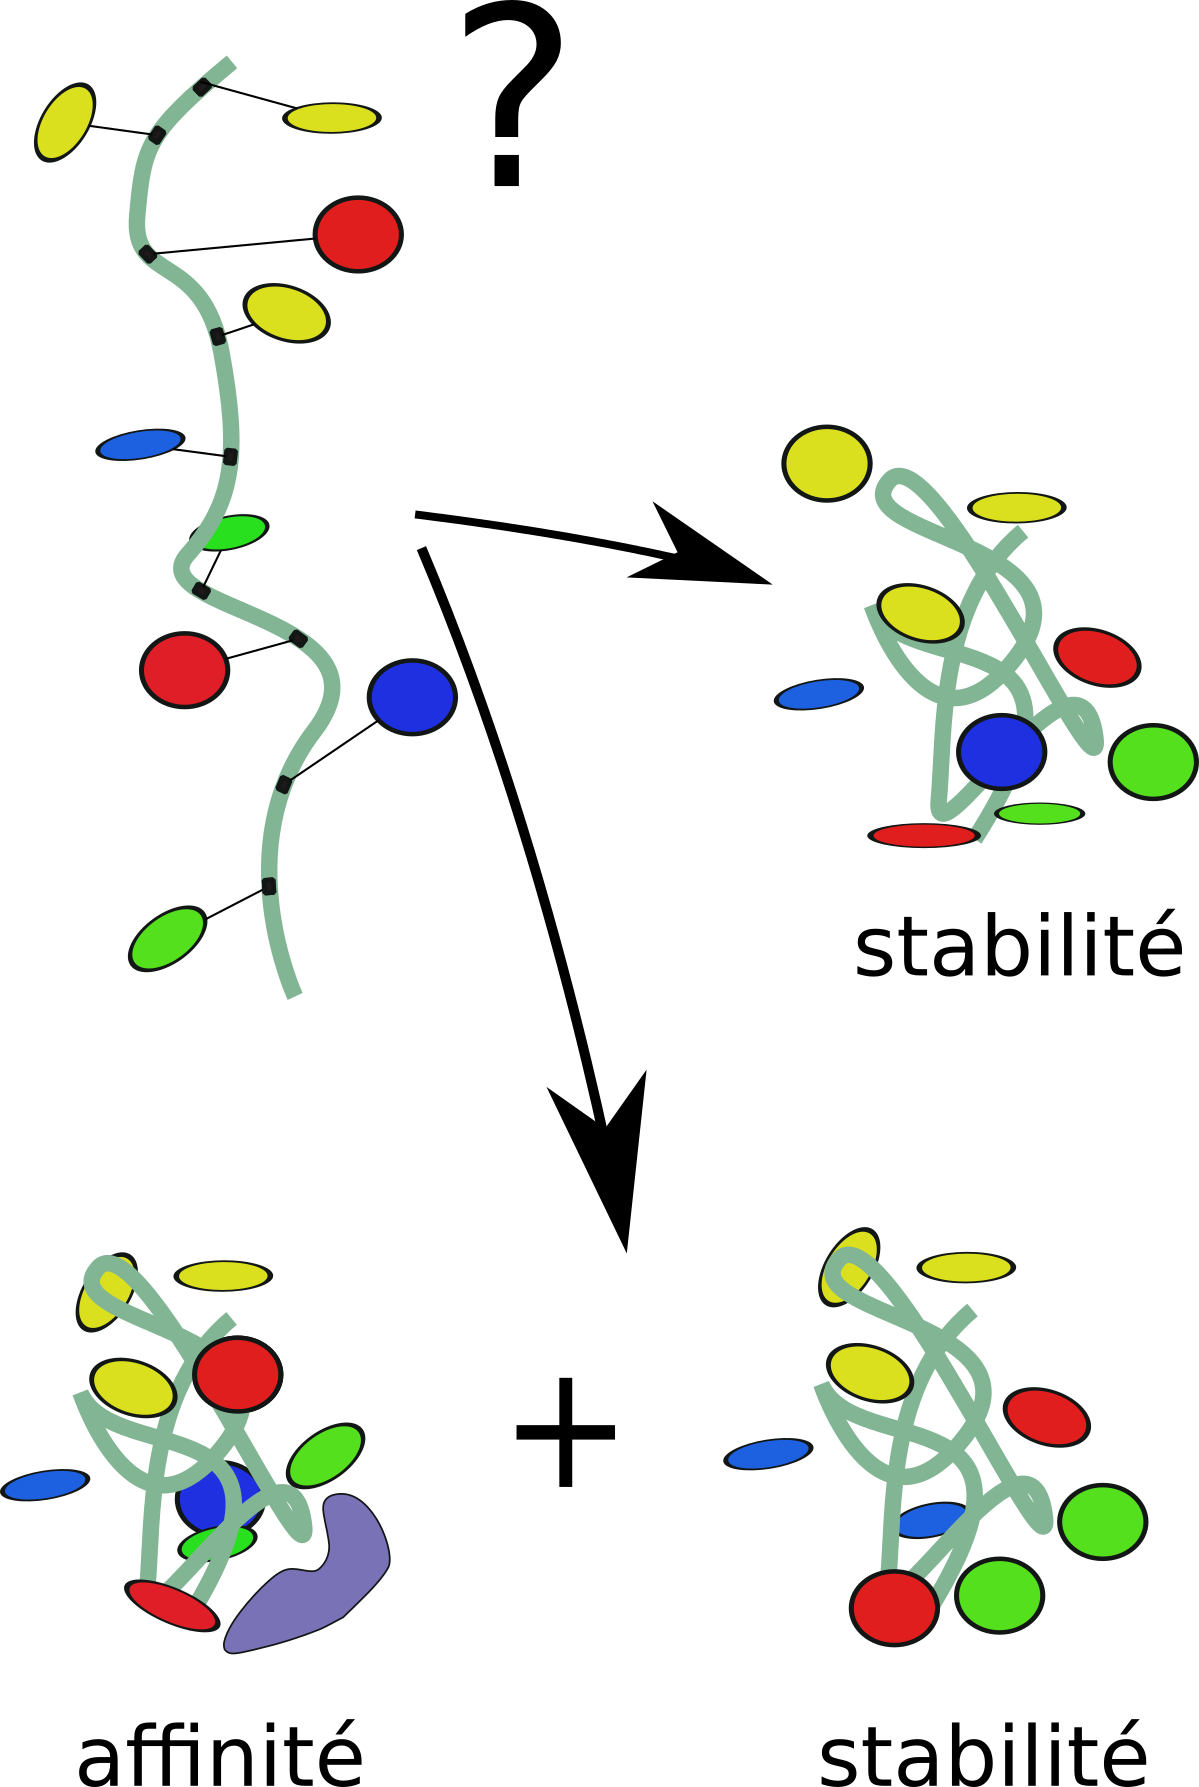
\includegraphics[width=7cm]{figure/CPD.png} &
     \end{tabular}
     
     \caption{Le CPD pour \og Computational Protein Design\fg recherche les séquences d'acides aminés compatibles avec une protéine dont la structure 3D  est connue, c'est-à-dire compatibles avec un repliement et éventuellement une affinité à un ligand.}
\label{graph:CPD}
   \end{figure}


\begin{enumerate}[leftmargin=*]

\item \textbf{La définition d'un espace de conformations de la protéine}\\
C'est sur elle que repose la prédiction de structure des séquences considérées. Elle doit inclure une ou plusieurs conformations de la chaîne principale du polypeptide et un ensemble de positionnements de la chaîne latérale de chaque résidu.
\item \textbf{Une fonction d'énergie}\\
Elle permet d'évaluer la pertinence des conformations. 
\item \textbf{Un algorithme d'exploration de l'espace de séquences-conformations}\\
Il exploite la fonction d'énergie pour échantillonner les séquences favorables.
\end{enumerate}

Dans la suite de ce chapitre, nous détaillons les trois composantes du CPD. Nous aborderons le problème de la modélisation des protéines, de leur espace de conformation et de l'espace séquences-conformations. Puis, nous verrons les fonctions d'énergies classiques. Seront détaillées les approches pour la modélisation du solvant qui est une partie importante de la fonction d'énergie. Plusieurs algorithmes d'exploration de l'ensemble des états possibles vont être abordés.  

\section{L'espace des séquences-conformations}
Pour faire du CPD, il faut une représentation de l'ensemble des conformations que les chaînes polypeptidiques peuvent adopter. L'ensemble des cas possibles peut se concevoir comme le choix d'une séquence $S$ d'acides aminés de longueur $N$ et la détermination d'une conformation $C$ prise par $S$ dans l'espace 3D. Ainsi l'espace d'états est celui des couples $(S,C)$ pour $N$ donné. Dans la suite, on appelle une séquence-conformation un élément de cet ensemble de couples. L'ensemble des séquences de $N$ acides aminés se conçoit sans difficulté comme les $N$-uplets de l'ensemble à $20$ éléments formé des différents types d'acide aminé. En revanche, la définition de l'ensemble des conformations d'une chaîne polypeptidique doit être développée.

\subsection{L'état replié }
\label{sec:etatreplie}
La mécanique moléculaire propose d'appliquer les représentations de la mécanique classique aux molécules. Les atomes sont représentés sous forme de sphères. La protéine dans un milieu aqueux est flexible et en permanence en mouvement. C'est en particulier le cas pour les chaînes latérales et les boucles flexibles. L'espace d'états d'une chaîne polypeptidique, dans le cadre de la mécanique moléculaire est alors constitué d'un vaste espace continu de conformation possibles.

D'autre part, si un domaine polypeptidique a un nombre N de résidus compris entre 50 et 100, et que chacune des N positions de la chaîne peut adopter l'un des 20 types d'acides aminés, le nombre de séquences à considérer est égale à  N$^{20}$. Il en résulte un espace des séquences-conformations trop grand pour être utilisable. Il faut donc réduire la taille de l'espace des conformations. Pour cela, Ponder et Richards \cite{Ponder87} proposent une approche en deux points:
\begin{enumerate}[leftmargin=*]
\item Le squelette de la protéine est fixé.
\item Les conformations des chaînes latérales sont réduites à un ensemble fini de positionnements possibles dans l'espace euclidien, les \og rotamères\fg.
\end{enumerate}  
Ensuite, des variations sur ce principe ont étés introduites, avec notamment la prise en compte de la mobilité de la chaîne principale dans un ensemble discret ou continu d'états. L'approche qui consiste à générer un ensemble de squelettes et à faire des calculs CPD pour l'ensemble a été utilisée par Su et Mayo \cite{Su97}. 
Présentons maintenant, la modélisation des chaînes latérales et celle du backbone, c'est-à-dire le squelette polypeptidique.

\subsubsection{Les chaînes latérales}

Finkelstein et Ptitsyn \cite{Finkelstein77}, Janin et al. \cite{Janin78} ainsi que Ponder et Rischards \cite{Ponder87} ont établi que la chaîne latérale des résidus adopte de façon préférentielle un petit ensemble de conformations. Janin introduit alors le terme de \og rotamère\fg pour désigner ces conformations. Il est alors possible de réduire l'espace continu des conformations des acides aminés à cet ensemble discret de rotamères. La plupart des méthodes de CPD utilisent cette discrétisation. Beaucoup de librairies de rotamères ont été proposées dans la littérature. La plupart sont indépendantes du backbone. Mais il existe également des librairies qui dépendent du squelette de la protéine voir \cite{McGregor87,Dunbrack93}. 

\subsubsection{Le squelette}
Comme le positionnement des chaînes latérales n'influence que faiblement la structure adoptée par le squelette, celui-ci est fixé dans beaucoup de programmes CPD. Le problème de la prédiction de structure est alors ramené à celui du placement des chaînes latérales sur ce squelette. De par la configuration particulière de la proline et de la cystéine avec le backbone, ces deux types sont souvent traités à part. Cette approche a obtenu de nombreux succès, voir par exemple \cite{Dahiyat97b}.

Cependant, cette approximation peut avoir des conséquences importantes. Un type d'acide aminé considéré comme défavorable peut devenir favorable après une petite adaptation du backbone et il a été établi que quelques mouvements de squelettes peuvent faire varier significativement l'énergie de la conformation \cite{Desjarlais99}.
En réponse à ce problème, Druart et al. \cite{Druart16} proposent une méthode de Monte Carlo hybride travaillant sur un modèle multi backbone. Une autre approche consiste à donner une certaine liberté aux angles $\Phi$, $\Psi$ en introduisant des variations aléatoires \cite{Desjarlais99}. Dantas et al. \cite{Dantas07} font des simulations avec minimisation après chaque mouvement de chaîne latérale. Kuhlman et al. \cite{Kuhlman03}  optimisent alternativement la structure du squelette et la séquence d'acides aminés.

Enfin, citons l'utilisation d'une classe particulière de mouvement des squelettes protéiques appelé \og backrub \fg. Ce sont des mouvements naturels du backbone mis en évidence par David et al. \cite{Davis06}, à partir de structures cristallographiques. Ces mouvements consistent en des déplacements de l'ensemble $C_{\alpha}-C_{\beta}$ à une position $i$ donnée de la chaîne, sans déplacement des carbones $C_{\alpha_{i+1}}$ et $C_{\alpha_{i-1}}$. Ces mouvements backrub ont permis \cite{Georgiev08,Smith08} d'améliorer la qualité des prédictions des mutants par rapport à des simulations à squelette rigide.

\subsection{L'état déplié }
\label{sub:deplie}
En général, la stabilité d'une protéine est évaluée par une variation de l'énergie libre entre son état déplié et son état replié. Il faut alors connaître l'énergie de l'état déplié. Mais cet état est déstructuré par définition et ne correspond pas à une conformation unique; la modélisation exhaustive est difficile. Une approche simple consiste à représenter cet état par une chaîne étendue dans laquelle un résidu de la protéine est en interaction principalement avec le solvant et avec le backbone. Ainsi l'énergie libre de l'état déplié dépend de la séquence uniquement par la composition en acides aminés de celle-ci. En pratique, on peut utiliser pour chaque type d'acide aminé X de la protéine  un tripeptide ALA--X--ALA, et on identifie son exposition au solvant à celle dans l'état déplié \cite{Dahiyat96}. On en déduit une énergie par type X que l'on somme sur la séquence pour obtenir l'énergie de la protéine dépliée. 

\section{L'énergie d'une protéine}

La fonction d'énergie permet d'évaluer la stabilité de chaque conformation de la protéine. Cette fonction doit prendre en compte les détails des interactions entre les atomes de la protéine, les effets de l'environnement aqueux et en même temps, être suffisamment rapide à calculer pour évaluer en un temps raisonnable une partie la plus significative possible de l'espace des conformations. Une classe importante est basée sur la mécanique moléculaire.

\subsection{La mécanique moléculaire}
\label{sub:mecamol}
La mécanique moléculaire représente les atomes comme des particules sphériques ayant une charge électrique nette fixe généralement placée au centre de la sphère et chaque liaison est modélisée par un ressort. Cette description, associée à un choix de paramètres numériques optimisés est appelée un champ de force. Ce champ de force décrit les interactions interatomiques du point de vue énergétique et est invariant au cours d'une simulation.
Dans toute la suite, nous appelons $E_{MM}$ l'énergie qui dérive d'un tel champ de force.

Il existe beaucoup de champs de force à la disposition des simulateurs. Quatre des principaux optimisés pour les protéines sont:

\begin{itemize}
\item AMBER: Assisted Model Building with Energy Refinement \cite{Cornell95}
\item CHARMM: Chemistry at HARvard Molecular Mechanics \cite{Brooks09}
\item OPLS: Optimized Potential for Liquid Simulations \cite{Jorgensen88}
\item GROMOS:GROningen MOlecular Simulation \cite{Christen05}
\end{itemize}
L'énergie d'une conformation se définit alors comme la somme de l'énergie $E_{MM}$  et de l'énergie de solvatation:
\begin{equation}
  E = E_{MM} + E_{solv}
\end{equation}
Le terme $E_{MM}$ se décompose à son tour en deux termes:
\begin{equation}
  E_{MM} = E_{liée} + E_{non\ liée}
\end{equation}
avec $E_{liée}$ l'énergie d'interactions des atomes éloignés d'au plus deux liaisons covalentes et $E_{non\ liée}$  l'énergie des autres interactions. Détaillons ces deux énergies.

\subsubsection{Les interactions liées }

L'énergie d'interaction liée comprend un terme d'élongation des liaisons, un terme de déformation des angles, de rotation des angles dièdres et un terme \og impropre\fg:
\begin{equation}
  E_{liée} = E_{liaison} + E_{angle} +E_{dièdre} + E_{impr}
\end{equation}
L'énergie de déformations des liaisons $E_{liaison}$ s'exprime de la façon suivante:
\begin{equation}
  E_{liaison} = \frac{1}{2} \sum_{i=1}^{n} k_{i} (r_i - r^o_i)^2
\end{equation}
avec l'ensemble des liaisons indexé par $i$, $k_{i}$ la force du ressort, $r_{i}$ la longueur de la liaison et $r^0_i$ la longueur optimale. L'énergie de déformation des angles $E_{angl}$ s'exprime:
\begin{equation}
  E_{angl} =\frac{1}{2} \sum_{ij}k_{\theta,ij}(\theta_{ij} - \theta_{ij}^0)^2
\end{equation}
avec $\theta_{ij}$ l'angle entre les liaisons $i$ et $j$, $\theta_{ij}^0$ l'angle optimal et $k_{\theta,ij}$ la force du ressort.
L'énergie de déformation des angles dièdres $E_{dièdre}$ s'exprime:
\begin{equation}
E_{dihe} = \frac{1}{2}\sum_{i} A_{i,n}[ 1 + \cos(n\Phi_i - \Phi_0)]
\end{equation}
où $n$ est périodicité de la rotation, $A_{i,n}$ est la constante de torsion, $\Phi_i$ l'angle dièdre, c'est-à-dire pour 4 atomes $a_1$, $a_2$, $a_3$ et $a_4$, reliés par 3 liaisons $a_1-a_2, a_2-a_3$ et $ a_3-a_4$, l'angle formé par les plans $(a_1,a_2$,$a_3)$ et $(a_2,a_3$,$a_4)$, $\Phi^0$ est la phase. L'énergie de déformation des angles impropres $E_{impr}$ exprime la déformation d'un  ensemble  de 4 atomes  par rapport à une conformation plane ou tétraédrique. Pour un atome $a_1$ relié à 3 atomes $a_2$,$a_3$ et $a_4$, elle a la forme:
\begin{equation}
  E_{impr}= \frac{1}{2}A(\omega - \omega^0)^2
\end{equation}
Ici, $A$ est la constante de force et $\omega$ représente l'angle entre les plans ($a_1$, $a_2$, $a_3$) et ($a_2$, $a_3$, $a_4$), voir la figure \ref{graph:Eliees} pour une représentation visuelle.

   \begin{figure}[!htbp]
     \centering
     \begin{tabular}{cc}
       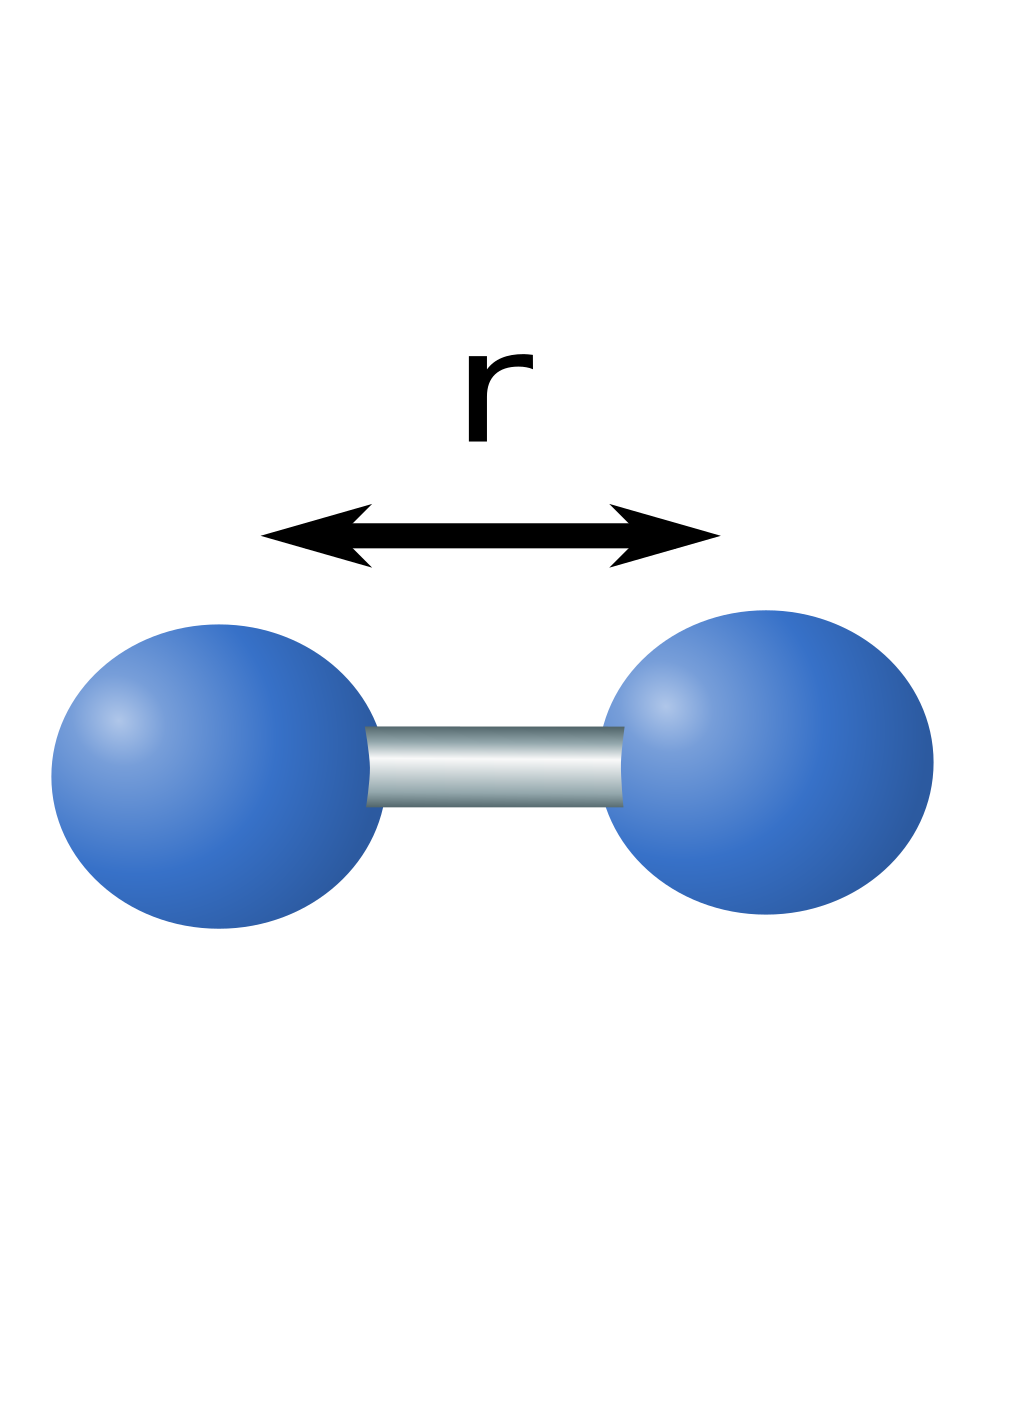
\includegraphics[width=3cm]{figure/liaison.png} &
       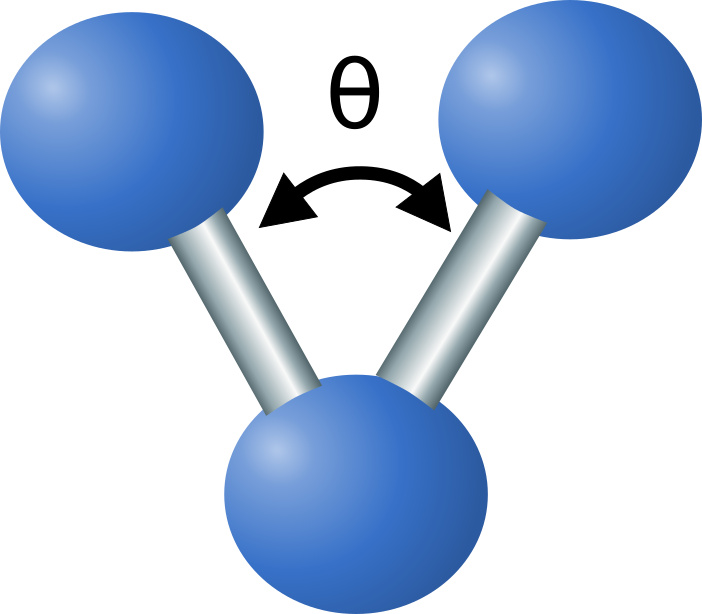
\includegraphics[width=3cm]{figure/angle.png} \\
       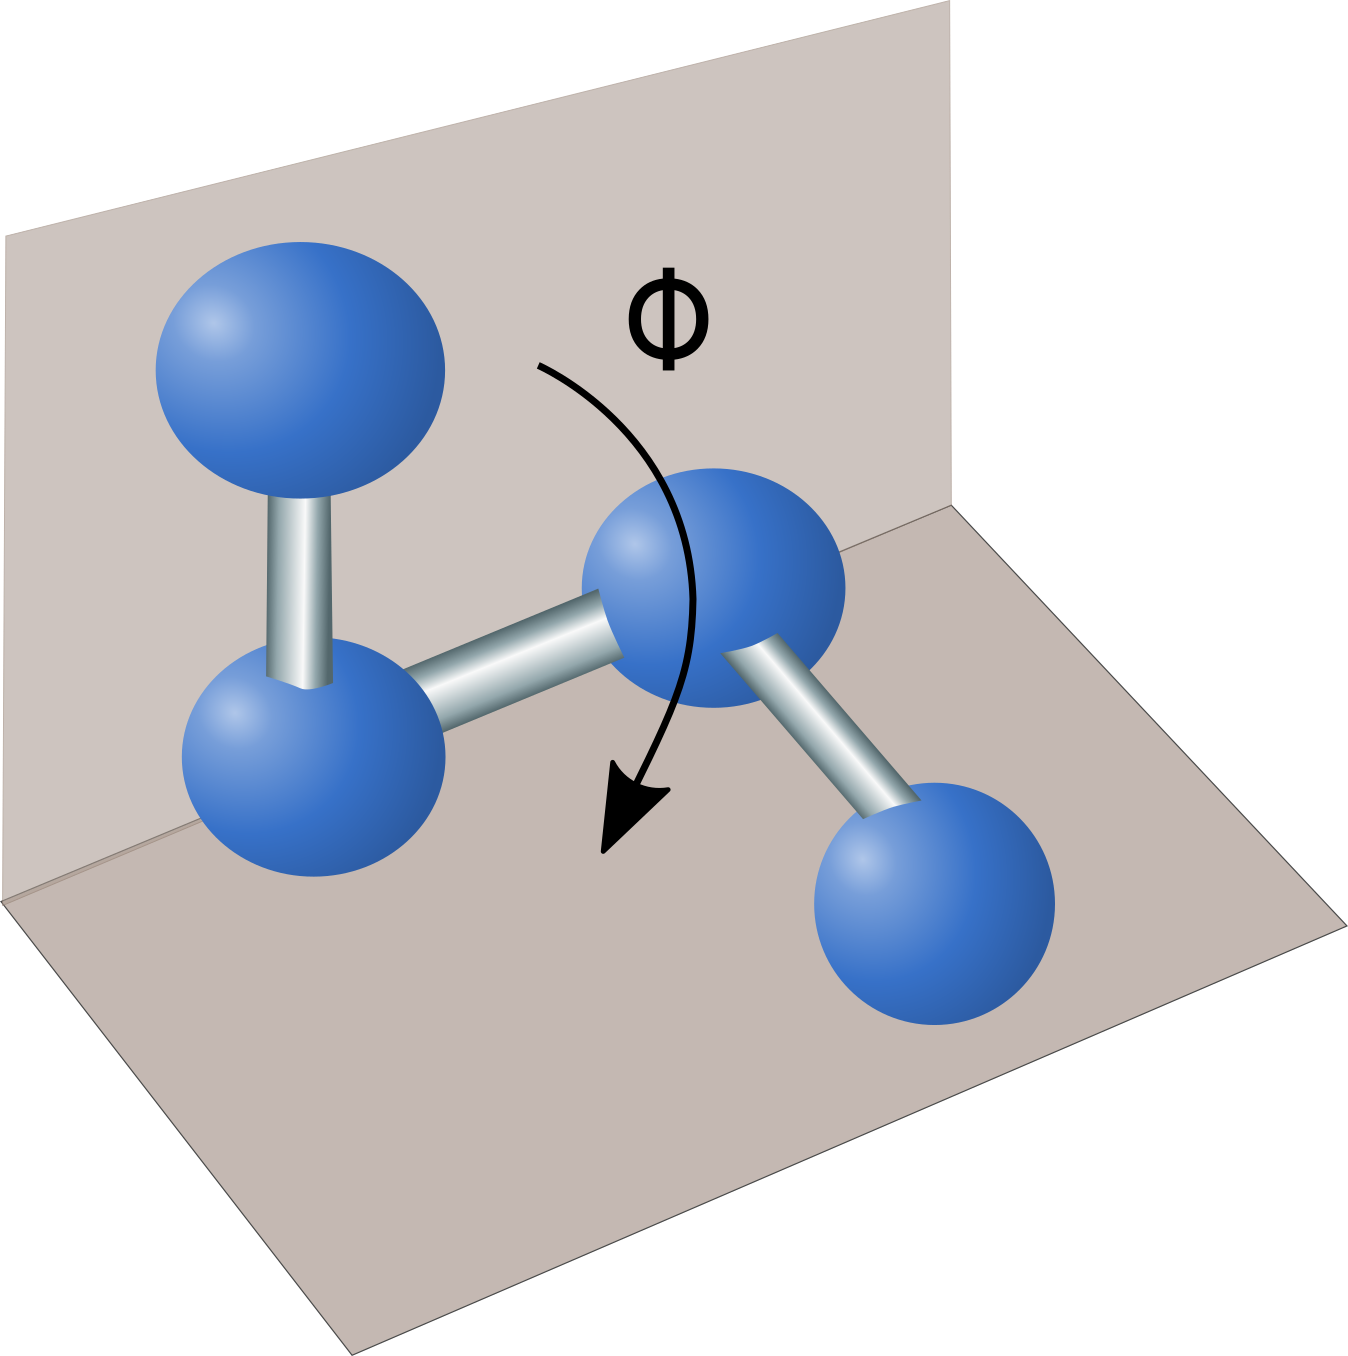
\includegraphics[width=5cm]{figure/dihedre.png} &
       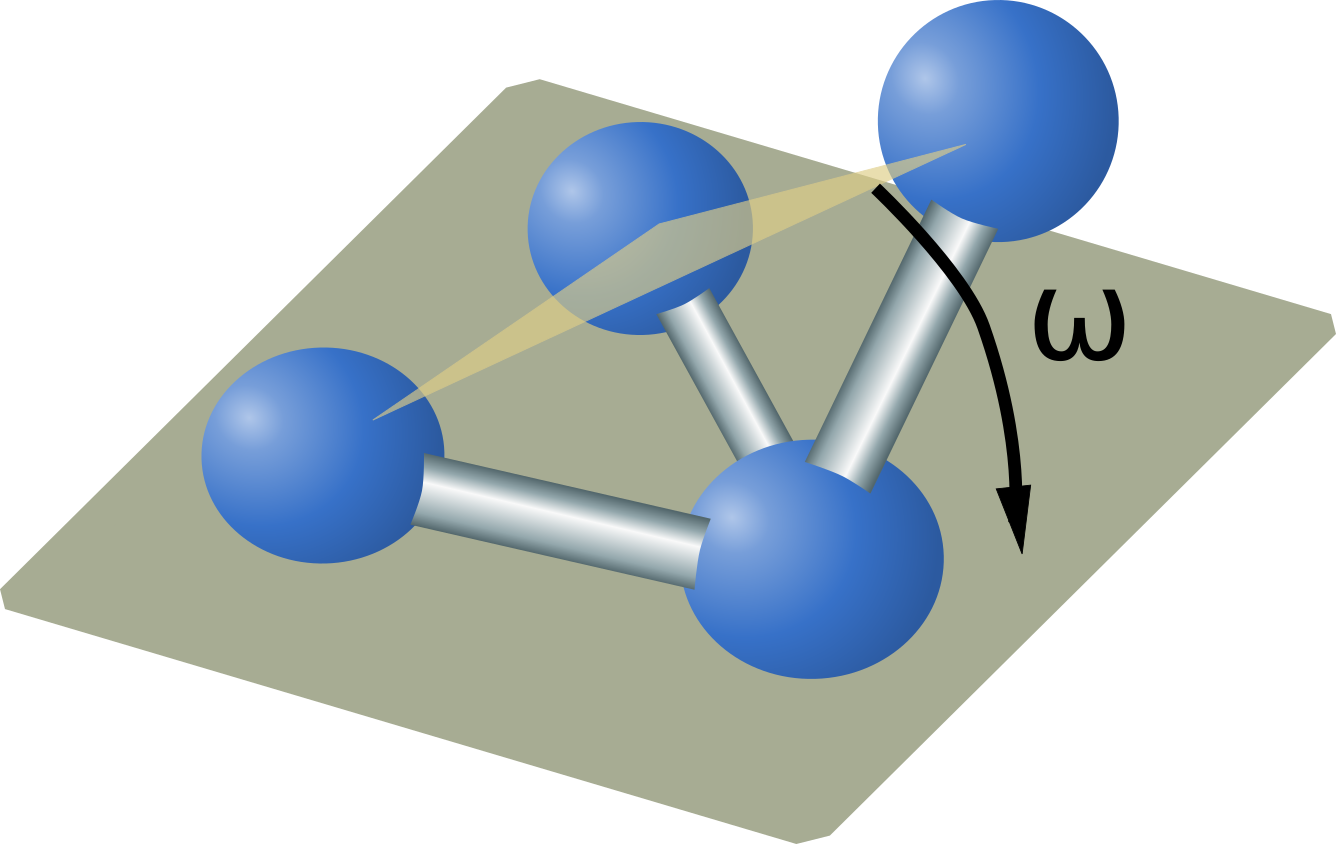
\includegraphics[width=5cm]{figure/impropre.png} \\

     \end{tabular}
     
     \caption{\textbf{Représentation des énergies liées} De la gauche vers la droite et du haut vers le bas, sont représentés les énergies de liaison, d'angle, du dièdre et du dièdre impropre.}
\label{graph:Eliees}
   \end{figure}

\subsubsection{Les interactions non liées}
Les interactions non liées sont les interactions entre atomes séparés par plus de trois liaisons covalentes ou qui appartiennent à des molécules différentes. Les interactions sont caractérisées par les deux termes suivants:
\begin{equation}
E_{non\ liées} = E_{elec} + E_{vdw}  
\end{equation}
L'énergie $E_{elec}$ pour l'énergie électrostatique est donnée par un potentiel de Coulomb de la forme:
\begin{equation}
  E_{elec}=\frac{q_iq_j}{\epsilon r_{ij}}
\end{equation}\\
$q_i$ et $q_j$ représentent les charges respectives des atomes $i$ et $j$ et $r_{ij}$ la distance entre les atomes $i$ et $j$, $\epsilon$ la constante diélectrique du milieu.

L'énergie  $E_{VdW}$ de Van der Waals s'explique par les interactions électriques de faible intensité entre deux atomes, dus au fait que la répartition des charges électriques n'est pas uniforme autour des noyaux. Elle rassemble les effets des forces de Keesom, Dedye, London et Pauli. Le potentiel de Lennard-Jones est l'approximation classique de cette énergie. Voici son expression:
\begin{equation}
    \label{VdW}
E_{vdw} = \sum_{i<j}D_0 [(\frac{r_0}{r_{ij}})^{12} - (\frac{r_0}{r_{ij}})^6]  
\end{equation}
avec $D_0$ et $r_0$ des constantes, $r_{ij}$ la distance entre l'atome $i$ et l'atome $j$. Le premier terme est répulsif à courte distance, ce qui représente l'évitement de l'encombrement stérique entre $i$ et $j$. Le second terme domine à grande distance, c'est un terme attractif. 
  

\subsection{D'autres approches}

Même si la mécanique moléculaire prédomine dans le monde du CPD, il existe d'autres approches. Zollars et al. utilisent une fonction empirique pour la modélisation des liaisons hydrogènes avec une fonction d'énergie de Coulomb qui contient un $\epsilon$ qui varie en fonction de la distance interatomique \cite{Zollars06}. Il existe des fonctions d'énergie comportant des éléments relevant de statistiques sur les protéines \cite{Pokala05}. Il existe encore des fonctions d'énergie à gros grains notamment dans la modélisation des forces de Van der Waals utiles pour les interactions protéine-protéine \cite{Korkut09}.

\section{La modélisation du solvant}
Les protéines sont étudiées dans un solvant aqueux. La solution qui est considérée dans les calculs est un mélange dans lequel l'eau est présente en quantité largement plus importante que la protéine. Bien qu'il existe d'autres types de solvant, ils ne sont pas abordés ici. Les interactions entre solutés et solvant jouent un rôle clé dans la structure de la protéine, mais également dans sa fonction. La modélisation du solvant est alors un point capital pour le CPD.

Une molécule d'eau a une charge électrique nette nulle. Mais il existe une dissymétrie du nuage électronique: les électrons se situent de façon préférentielle au voisinage du noyau de l'oxygène par rapport à ceux des deux noyaux d'hydrogènes. On dit que la molécule est polaire, et cette polarisation peut être approchée par un moment dipolaire. Cette polarité permet la formation de liaisons hydrogènes entre molécules d'eau et avec tout autre groupe polaire. Ainsi, l'eau à l'état liquide possède beaucoup de liaisons hydrogènes.

Lorsqu'une protéine est solvatée, les molécules du solvant se placent de telle façon que le nombre de liaisons hydrogène soit maximal. Les molécules de la première couche de solvatation forment alors des liaisons avec les groupes polaires de la protéine, près des groupes non polaires, s'orientent pour former des liaisons avec d'autres molécules d'eau. Cette réorganisation de la structure moléculaire de l'eau a trois conséquences importantes:

\begin{itemize}
\item Une diminution de l'entropie au voisinage de la protéine  
\item La création de polarisation à la surface du soluté
\item  L'eau crée une couche de charges partielles opposées à celles de la protéine qui atténue le champ de celle-ci. Ce phénomène s'appelle l'écrantage.
\end{itemize}
  
Il a été démontré qu'une protéine et une molécule d'eau peuvent interagir de façon non négligeable jusqu'à une distance de 15 Angströms. Cela implique que pour solvater correctement une protéine, il faut prendre en compte l'effet de plusieurs milliers d'atomes du solvant.
De nombreuses méthodes ont été développées pour faire face à la difficulté que cela représente.
La connaissance des positions et les vitesses des atomes de toutes les molécules d'eau nécessaire dans le cadre de la mécanique moléculaire, apparaît alors comme une gageure. Des approches moins fines doivent être utilisées. 

\subsection{Le modèle de solvant explicite}

Pour calculer les grandeurs d'intérêt du solvant, il faut pouvoir situer le système dans l'espace des phases, un espace à $6\,N$ dimensions pour une simulation du solvant avec $N$ molécules d'eau.
Une première méthode est la dynamique moléculaire dans laquelle, à partir d'une configuration initiale des molécules d'eau, les équations de la mécanique classique sont résolues pour déterminer les positions et les vitesses au cours du temps. Une seconde méthode consiste à échantillonner l'espace des phases par la méthode Monte Carlo dans laquelle l'espace est visité grâce à une série de déplacements aléatoires qui sont acceptés ou non en fonction de critères basés sur l'énergie (voir la section \ref{sub:MC}).

Quelle que soit la méthode utilisée, pour pouvoir obtenir une représentation de qualité des effets du solvant sur la protéine, il faut échantillonner correctement les états du solvant dans l'espace des phases, ce qui demande de multiplier les dynamiques moléculaires avec différentes configurations initiales ou de calculer des trajectoires Monte Carlo suffisamment longues.
L'utilisation d'un modèle de solvant explicite entraîne alors une situation dans laquelle une simulation très coûteuse en termes de puissance de calculs consacre la plus grande partie du temps à évaluer des interactions entre des molécules d'eau. Ce n'est pas un objectif pour le CPD.

\subsection{Le modèle implicite}

Le principe des modèles implicites du solvant est de représenter l'effet moyen du solvant sur la protéine par l'utilisation d'un milieu continu dans lequel la protéine serait immergée. Le solvant et la protéine sont représentés chacun par un milieu diélectrique uniforme.
Pour mesurer l'effet de la solvatation, la bonne quantité est l'énergie libre de solvatation mise en jeu pendant ce processus. Elle se définit comme la différence entre l'énergie libre de la solution et l'énergie libre d'un système dans lequel le solvant et le soluté sont séparés et à l'état pur. Notons cette différence $\Delta G_{solv}$. On peut décrire $\Delta G_{solv}$ comme la somme de trois termes:

\begin{equation}
  \label{eq:enersolv}
  \Delta G_{solv} = \Delta G_{solv}^{elec} + \Delta G_{solv}^{vdw} + \Delta G_{solv}^{cav}
\end{equation}
avec:

\begin{itemize}
\item $\Delta G_{elec}$ l'effet électrostatique, qui correspond à la réorganisation des charges de la protéine dans le solvant, y compris ses charges partielles (polarisation).
\item $\Delta G_{vdw}$ est l'effet des forces de Van der Waals.
\item $\Delta G_{cav}$ est l'effet qui correspond au coût de la création de la cavité, en termes d'entropie et de pression. Il inclut le coût de réorganisation des molécules du solvant.
\end{itemize}

Une méthode standard pour approcher $\Delta G_{solv}$ est de traiter le premier terme séparément des autres. En effet, il est possible d'approcher la somme des deux derniers termes de l'équation  \ref{eq:enersolv} en utilisant la surface accessible au solvant de la protéine. Cette surface est l'ensemble des points par lesquels peut passer le centre d'une sphère, modélisant une molécule d'eau, qui roule sur la surface de Van der Waals de la protéine, voir figure \ref{graph:surface}. L'approximation s'écrit:
\begin{equation}
  \label{eq:SA}
\Delta G_{solv}^{vdw} + \Delta G_{solv}^{cav} \approx E_{solv}^{surf} = \sum_i \sigma_{t_i} A_i
\end{equation}
avec $A_i$ la surface accessible au solvant de l'atome $i$  et $\sigma_{t_i}$ un facteur pour chaque type atomique $t_i$ ajusté pour retrouver les énergies de solvatation obtenues par expérience.
Dans la suite, on appelle cette somme, le terme surfacique de l'énergie de solvatation, et on le note $E_{solv}^{surf}$.

   \begin{figure}[!htbp]
     \centering
     \begin{tabular}{c}
       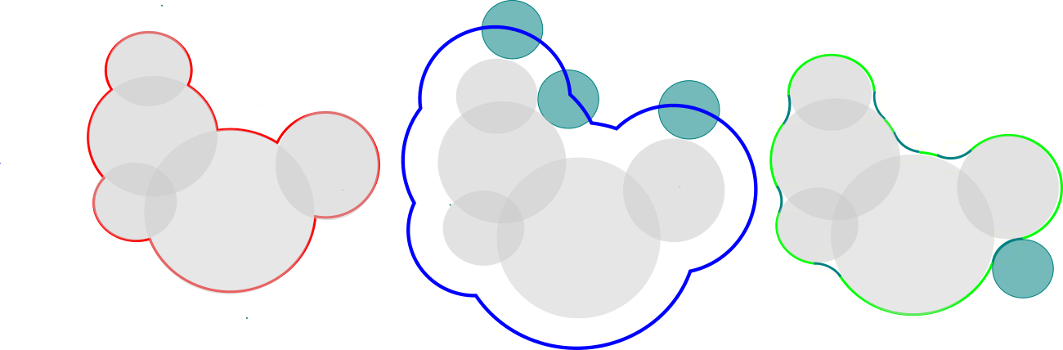
\includegraphics[width=13cm]{figure/surface.png} &
     \end{tabular}
     
     \caption{\textbf{Les trois types classiques de surfaces pour une molécule} À gauche et en rouge la surface de Van der Waals (SVdW), au centre et en bleu, la surface accessible au solvant (SA), à droite, et en vert  la surface de Connolly ou surface moléculaire (SM). La surface SA est l'ensemble des positions pouvant être occupées par le centre d'une sphère (figurant une molécule du solvant) roulant sur SVdW. La surface SM est la plus petite enveloppe de SVdW dont chaque point peut être en contact avec la sphère. } 
\label{graph:surface}
   \end{figure}
   

\subsection{Le modèle CASA}
\label{sub:CASA}
Pendant la réorganisation du solvant, les molécules d'eau s'orientent, au moins pour les plus proches du soluté, selon les lignes du champ électrique créé par la protéine, voir figure \ref{graph:ecrantage}. L'idée du modèle \og Coulomb accessible surface area\fg (CASA) est alors de considérer que l'effet électrostatique induit par le solvant est proportionnel à l'effet électrostatique produit par la protéine. On a  alors, en utilisant le modèle \texblt{SA} pour le terme surfacique:

\begin{equation}
\Delta G_{solv} \approx E_{screen} + \sum_i \sigma_{t_i} A_i
\end{equation}
avec 
\begin{equation}
E_{screen} =  (\frac{1}{\epsilon} -1 )E_{coul}
\end{equation}
et $ \epsilon $ la constante diélectrique du solvant. Ainsi, l'effet du solvant est décrit par un facteur unique pour toutes les interactions électrostatiques. La simplicité de ce modèle proposé par Wesson et Einsenberg \cite{Wesson92} fait de lui un modèle fréquemment utilisé. Cependant, il est en difficulté pour le traitement de la surface des protéines.


   \begin{figure}[!htbp]
     \centering
     \begin{tabular}{c}
       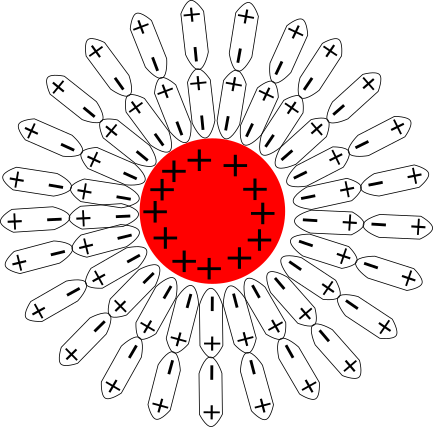
\includegraphics[width=6cm]{figure/ecrantage.png} &
     \end{tabular}
     
     \caption{\textbf{Représentation schématique de l'organisation des dipôles des molécules d'eau autour d'un soluté sphérique chargé positivement à sa surface}. Les dipôles des premières couches de solvatation s'orientent suivant les lignes du champ électrique produit par le soluté.}
\label{graph:ecrantage}
   \end{figure}
   
\subsection{Le modèle Poisson-Boltzmann}
La méthode de Poisson-Boltzmann est très utilisée parce qu'elle prend en compte l'effet ionique et toute la forme de la protéine. Dans cette méthode, la protéine est supposée fixe, elle forme une cavité dans un milieu continu diélectrique qui peut être polarisé (on parle de continuum), il s'agit donc encore d'un modèle de solvant implicite. Ainsi le modèle prend en compte l'écrantage par le solvant et les interactions électrostatiques entre groupes chargés de la protéine et du solvant polarisé. Si le continuum est muni d'une distribution de charge $\rho$ alors le potentiel électrostatique dans ce milieu est donné par l'équation de Poisson:

\begin{equation}
  \label{eq:poisson}
  \nabla [ \epsilon(x) \phi(x)] = - 4 \pi \rho(x)   
\end{equation}
avec $\epsilon(x)$ la constante diélectrique (ici c'est une fonction à deux valeurs possibles selon le milieu), $\phi (x)$ le potentiel électrostatique, $\nabla \phi(x)$ la divergence de $\phi$ en $x$.
Typiquement $\epsilon$ prend une valeur faible, entre $1$ et $8$ pour la protéine et élevée pour le solvant, proche de $80$.

L'équation de Poisson-Boltzmann est une extension de l'équation de Poisson dans laquelle les charges d'ions mobiles sont prises en compte. La théorie de Debye-Hückel donne la distribution des ions comme suivant une loi de Boltzmann, conduisant à:
\begin{equation}
  \nabla [ \epsilon (x) \phi(x)] = -4 \pi ( \rho(x) - \epsilon(x) \kappa^2 \phi(x))
\end{equation}
avec $ \kappa $ le paramètre de Debye-Hückel qui tient compte de la concentration des ions en solution.

Malheureusement, il n'existe pas, pour les protéines, de solution analytique à \ref{eq:poisson}. Il faut effectuer une résolution numérique. Plusieurs programmes sont à la disposition de la communauté, on peut citer Delphi \cite{Rocchia02} et APBS \cite{Baker01}  qui sont basés sur la méthode des différences finies et des éléments finis. Une fois l'équation résolue, le terme électrostatique de l'énergie de solvatation est donné par:

\begin{equation}
\Delta G_{solv}^{elec} = \frac{1}{2} \int \rho(x)\phi(x)dx  
\end{equation}
Quelle que soit l'approche utilisée, les calculs sont coûteux pour une protéine entière.


\subsection{Le modèle de Born Généralisé}
\label{sub:GB}
Dans le cas d'un soluté sphérique de rayon $a$ et de charge ponctuelle $q$ portée par le centre de la sphère, Born en 1920 \cite{Born20} établit des expressions analytiques des solutions de l'équation de Poisson-Boltzmann et de $ \Delta G_{solv}^{elec}$:
\begin{equation}
  \label{eq:Born}
  \Delta G_{solv}^{elec} = - \tau \frac{q^2}{2a}
\end{equation}
avec $ \tau = \frac{1}{\epsilon_p} - \frac{1}{\epsilon_s}$ , $\epsilon_p$ la constante diélectrique de la sphère et $\epsilon_s$ celle du solvant. Partant de cette solution en 1990, Still et al. \cite{Still90} proposent une généralisation à un ensemble d'atomes chargés formant une cavité de forme quelconque. L'objectif est de donner les résultats de qualité proche de celles de PB avec un coût numérique bien inférieur.

Dans un premier temps, on évalue l'énergie libre électrostatique totale d'une paire d'atomes $i$, $j$ de rayon $a_i$, $a_i$ de charge $q_i$, $q_j$ séparés d'une distance $r_{ij}$, en utilisant la solution de Born:
\begin{equation}
  \label{eq:GB}
  G_{elec} =  E_{Coul} + \Delta G_{solv}
\end{equation}
ce qui donne, si les particules sont éloignées;
\begin{equation}
  \label{eq:GB2}
  G_{elec} =  \frac{1}{2}  \frac{q_iq_j}{\epsilon_s r_{ij}} - \frac{1}{2}  \tau ( \frac{q_i^2}{a_i} +  \frac{q_j^2}{a_j})  
\end{equation}
ou, si $i=j$:
\begin{equation}
  G_{elec} = - \tau \frac{q_i^2}{2a_i}
\end{equation}
avec $ \tau = \frac{1}{\epsilon_p} - \frac{1}{\epsilon_s}$, $\epsilon_p$ la constante diélectrique des particules $i$ et $j$ et $\epsilon_s$ celle du solvant. L'idée consiste alors à étendre la somme des deux derniers termes de \ref{eq:GB2} aux distances $r_{ij}$ intermédiaires:

\begin{equation}
  G_{elec} = \frac{1}{2} \frac{q_iq_j}{\epsilon_s r_{ij}} - \tau \frac{1}{2} g_{ij}
\end{equation}
La forme des $g_{ij}$ la plus communément utilisée est la forme paramétrique suivante:


\begin{equation}
  \label{eq:GBg}
  g_{ij}= \tau q_iq_j (r^2_{ij} + b_ib_j exp(\frac{-r^2_{ij}}{4b_ib_j}))^{-1/2} 
\end{equation}
avec $b_i$ et $b_j$, de nouveaux paramètres, que l'on nomme les rayons de solvatations des atomes $i$ et $j$. Dans le cas où $i=j$, $g_{ij}$ est égale à deux fois l'énergie de solvatation de Born pour un ion de rayon $b_i$. Lorsque $r_{ij}$ tend vers l'infini, $g_{ij}$ tend vers la loi de Coulomb dans le solvant: $\frac{q_iq_j}{\epsilon_s r_{ij}}$. On écrit finalement pour une protéine constituée de $N$ atomes:

\begin{equation}
  G_{elec} = \frac{1}{2} \sum_{i \neq j} \frac{q_iq_j}{\epsilon_sr_{ij}} - \tau \frac{1}{2} \sum_{i,j}^N g_{ij}
\end{equation}


   \begin{figure}[!htbp]
     \centering
     \begin{tabular}{c}
       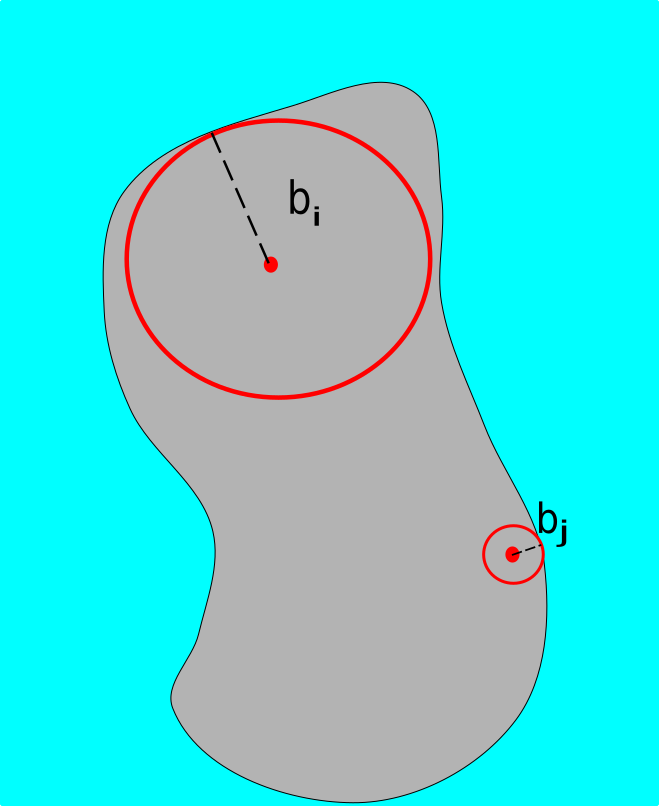
\includegraphics[width=6cm]{figure/rayon_Born.png} &
     \end{tabular}
     
     \caption{\textbf{Des rayons de Born de deux atomes dans une protéine} Le rayon de Born pour l'atome enfui est environ le rayon de la protéine, alors que le rayon de Born d'un atome à la surface est environ son rayon de Van der Waals.} 
\label{graph:rayonBorn}
   \end{figure}

Il reste à choisir une approximation pour les rayons de Born. La méthode classique se fait par l'énergie libre électrostatique de l'atome $i$, dans la situation où toutes les autres particules ont une charge ramenée à zéro. Ainsi, chaque charge de la protéine est caractérisée par sa distance au solvant, voir la figure \ref{graph:rayonBorn}. Alors, ce modèle permet le calcul de l'énergie libre de solvatation électrostatique à partir de la seule connaissance du volume de la protéine. En revanche, comme ces $b_i$ sont fonction de la position relative à $i$ de tous les atomes de la protéine, ils dépendent de sa conformation:
\begin{displaymath}
b_i=b_i(r_1,r_2,..,r_N)
\end{displaymath}
Ainsi, l'interaction entre une paire $i$ et $j$ dépend des postions de tous les atomes.
\paragraph{\og Native Environnement Approximation\fg (NEA)}
\label{NEA}
Dans la variante NEA pour \og Native Environnement Approximation \fg  du modèle GB, le rayon de solvatation des atomes de chaque chaîne latérale est calculé avant l'étape d'exploration, en fixant tout le reste du système dans sa séquence native et sa conformation native \cite{Polydorides11,Simonson13,Gaillard14}. Par la suite, les $b_i$ ont des valeurs constantes, qui ne dépendent pas de la conformation. Ainsi $G_{elec}$ prend la forme d'une somme de termes qui ne dépendant chacun que d'une paire d'atomes $i$, $j$: on dit qu'elle est \og décomposable par paires\fg.

\section{L'algorithme d'exploration}

Il reste à déterminer un algorithme d'exploration de l'espace d'états qui permet la sélection d'un sous-ensemble de séquences les plus pertinentes. L'objectif du CPD est d'obtenir l'ensemble des séquences d'acides aminés compatibles avec une structure 3D ou qui réalisent une fonction donnée. Un tel algorithme a pour grand défi de faire face à l'immensité de l'espace d'états. On peut classer les différentes approchent utilisées en deux groupes.

Le premier groupe est constitué des méthodes déterministes dans lesquelles les choix effectués sont toujours déterminés a priori ou déterminés en fonction des éléments obtenus au cours de l'exécution du programme. On trouve par exemple dans ce groupe, les méthodes exhaustives qui exhibent la totalité des solutions du problème. Elles peuvent être appliquées à de petites espaces conformationnels. On trouve aussi des méthodes dites semi-exhaustives dans lesquelles la complexité combinatoire est réduite en autorisant uniquement certaines conformations à certains moments de l'exploration.

Une classe intéressante d'approches déterministes est constituée des algorithmes exacts qui se focalisent non pas sur l'objectif du CPD, mais sur la conformation de meilleure énergie ou \og Global Minimum Energy Conformation \fg (GMEC). Typiquement, ces algorithmes exploitent les structures de la fonction d'énergie et de l'espace d'états. Un type de méthodes est alors exploitable pour un type de fonction d'énergie. Bien souvent, ces algorithmes nécessitent également la discrétisation de l'espace des phases. Cela peut devenir problématique dans les situations où le backbone est flexible.
  
Le second groupe est celui des méthodes stochastiques et/ou heuristiques. Elles ont vocation à déterminer des solutions de qualité sans obtenir de garantie sur l'optimum en termes d'énergie, dans un temps d'exécution réaliste. Elles sont non-déterministes c'est-à-dire qu'elles choisissent certains éléments de façon aléatoire, en pratique la \og source de hasard\fg est constituée de générateurs de nombres pseudo-aléatoires. Elles permettent des espaces d'états non discrétisés, par exemple \cite{Perry12} où les rotamères peuvent varier de façon continue. Plusieurs peuvent s'utiliser sans exiger de structure particulière pour la fonction d'énergie. Par contre, la convergence bien qu'elle puisse être établie en théorie, reste en pratique difficile à cerner et n'offre pas la possibilité de reconnaître le GMEC. On doit au besoin choisir une condition d'arrêt de l'exécution sans lien direct avec ce minimum.  

Pour rendre possible l'utilisation de plusieurs outils algorithmiques, la fonction d'énergie doit être décomposable par paires, c'est-à-dire qu'elle doit être décomposable en une somme sur des paires de résidus. L'énergie d'une conformation C a alors la forme:
\begin{equation}
  \label{eq:pairwise}
E(C) = \sum_i E_i(r_i) + \sum_{i\neq j} E_{ij}(r_i,r_j)
\end{equation}
avec $r_i$ et $r_j$ les rotamères de la conformation C aux résidus $i$ et $j$, $E_i(r_i)$ l'énergie propre de $r_i$ et $E_{ij}(r_i,r_j)$ l'énergie d'interaction entre $r_i$ et $r_j$.

À présent, nous présentons quelques algorithmes parmi les plus utilisés.

\subsection{L'algorithme du champ moyen}
La méthode du champ moyen substitue l'ensemble des interactions entre un rotamère $r_0$ et les autres rotamères par une interaction unique moyenne. Pour calculer une interaction moyenne, la probabilité de Boltzmann est utilisée de la façon suivante. On note $P(r_{i})$ la probabilité que la chaîne latérale à la position $i$ soit dans le rotamère $r_i$. On a:
\begin{equation}
  \label{eq:CM1}
P(r_i) =\frac{\exp(-\beta E(r_{i}))}{\sum_{l_i=1}^{N_i} \exp(-\beta E(l_i))}}
\end{equation}
avec $N_i$ le nombre total de rotamères à la position $i$, et $\beta = \frac{1}{kT}$,  $k$ étant la constante de Boltzmann et $T$ la température.

Si on se limite au cas où une énergie d'interaction pour un résidu est la somme des interactions avec les autres résidus de la chaîne (énergie décomposable par paires), alors l'énergie d'interaction moyenne en $i$ est la somme des interactions impliquant le rotamère $r_i$ pondéré par le poids de Boltzmann de l'autre rotamère, c'est à dire:
\begin{equation}
    \label{eq:CM2}
E(r_i) = \sum_{i \neq j} \sum_{l_j}^{N_j} E(r_i,l_j)P(l_j)
\end{equation}  
avec $l_j$ parcourant tous les rotamères aux positions autres que $i$.

Les formules \ref{eq:CM1} et \ref{eq:CM2}, constituent un système itératif. Ainsi, l'algorithme se déroule de la façon suivante:
\begin{enumerate}[leftmargin=*]
\item  A chaque position, les rotamères sont équiprobables.
\item  Les énergies moyennes sont calculées grâce à la formule \ref{eq:CM2}.
\item  De nouvelles probabilités de Boltzmann sont calculées à partir des énergies moyennes précédentes et la formule \ref{eq:CM1}.
\item  Retour à l'étape 2 jusqu'à convergence des énergies.
\end{enumerate}
Cette méthode garantit la convergence vers un ensemble de rotamères stables à chaque position placée dans son \og environnement moyen\fg . Le temps de calcul avec cet algorithme augmente  de façon linéaire avec le nombre de résidus de la protéine, ce qui en fait un des algorithmes les plus rapides.

\subsection{Le Dead-End Elimination}
Le \og Dead End Elimination\fg (DEE)  consiste à éliminer des rotamères ou des combinaisons de rotamères qui ne peuvent pas faire partie de la conformation qui minimise l'énergie ou GMEC. Comme pour le champ moyen, l'énergie doit être décomposable par paires. Il y a deux critères d'élimination \cite{Desmet92}:

\textbf{Le critère simple:} le rotamère $r_i$ du résidu $i$ est éliminé si la meilleure énergie (la plus faible) qu'il est possible d'obtenir pour une conformation comprenant ce rotamère est moins bonne que la pire énergie obtenue avec un rotamère $r_i'$  à la même position. Notons $E(c)$, l'énergie d'une séquence-conformation $C$. Une expression mathématique de ce critère peut être le suivant:\\
Si $\displaystyle \min_{C;\,r_i \in C }E(C) > \max_{C;\, r_i' \in C} E(C)$ alors $r_i$ est éliminé. \\
En utilisant l'expression d'une fonction d'énergie décomposée par paires (équation \ref{eq:pairwise}), avec $N$ le nombre de positions, le critère peut s'écrire de la façon suivante:\\
Si $\displaystyle E_i(r_i) + \sum_{j\neq i} \min_{r_j} E_{ij}(r_i,r_j) > E_i(r_i') + \sum_{j\neq i}^{N} \max_{r_j}E_{ij}(r_i',r_j)$ alors $r_i$ est éliminé.\\ 

\textbf{Le critère double:} il exprime une condition analogue sur un couple de rotamères $(r_i,r_j)$ suffisante pour qu'il ne puisse pas faire partie du GMEC. Pour son expression on introduit l'énergie d'une paire $r_i$ , $r_j$: $E^{r_i,r_j} = E_i(r_i) + E_j(r_j) + E_{ij}(r_i,r_j)$. Il s'exprime ainsi comme suit:\\
Si\\
$\displaystyle E^{r_i,r_j} + \sum_{k=1}^N \min_{r_k} (E_{ik}(r_i,r_k) + E_{jk}(r_j,r_k)) >  E^{r_i',r_j'} + \sum_{k=1}^N \max_{r_k} (E_{ik}(r_i',r_k) + E_{jk}(r_j',r_k))$ \\
alors la paire $r_i$, $r_j$ est éliminée.\\
L'élimination d'un couple $(r_i,r_j)$, n'exclut pas pour autant la présence de $r_i$ ou de $r_j$ dans la solution optimale. 

\textbf{Le critère de Goldstein \cite{Goldstein94}:} il s'agit d'une amélioration du critère simple du DEE, voir la figure \ref{fig:DEE}. Il peut exister des situations dans lesquelles l'énergie avec un rotamère $r_i$  est toujours diminuée en la remplaçant par un autre rotamère $r'_i$. On peut donc l'éliminer. Or, cela n'implique pas forcément la condition du critère simple. Ce nouveau critère peut s'exprimer de la façon suivante:\\
S'il existe $r_{i'}$ tel que $\displaystyle E_i^{r_i} - E_i^{r_{i'}}+ \sum_{k=1}^N \min_{r_k} (E_{ik}(r_i,r_k) - E_{i'k}(r_i',r_k)) > 0$ alors $r_i$ est éliminé.

   \begin{figure}[!htbp]
     \centering
     \begin{tabular}{c}
       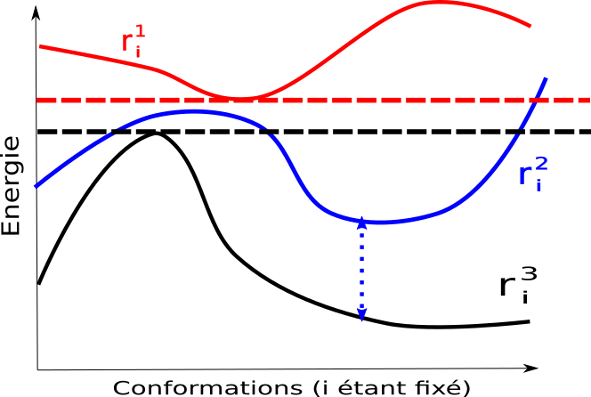
\includegraphics[width=8cm]{figure/DEE.png} &
     \end{tabular}
     
     \caption{\textbf{DEE, graphes de la fonction d'énergie pour des rotamères fixés à la position $i$} Le critère simple permet l'élimination du rotamère $r^1_i$ parce que l'énergie des conformations qui le contiennent, l'énergie rouge, est toujours moins bonne que la noire. Mais seul de critère de Goldstein permet d'éliminer $r^2_i$ parce que l'écart entre le graphe bleu et le graphe noir est positif pour chaque conformation.}
\label{fig:DEE}
   \end{figure}

Au cours de l'optimisation, les deux critères peuvent être utilisés alternativement, jusqu'à ce qu'il n'y est plus de rotamère à éliminer. Il est alors possible d'utiliser une approche exhaustive sur l'espace d'états réduit pour obtenir le GMEC. Cette méthode permet dans les bons cas (par exemple pour les petits systèmes) de converger en un temps raisonnable \cite{Leach98}. Beaucoup de variantes du DEE \cite{Pierce00,Lilien05} ont été proposées notamment en travaillant sur des combinaisons de plus de deux rotamères.


\subsection{Le CFN ou \og Cost Function Network\fg}

La méthode des réseaux de fonctions de coût est issue du domaine de l'optimisation combinatoire. Elle est utilisable si la fonction d'énergie est décomposable par paires. Il s'agit avant tout d'une recherche de la séquence-conformation qui minimise l'énergie globale ou GMEC. Dans certaines conditions, elle peut également fournir un ensemble de séquences-conformations proches du GMEC.

Un réseau de fonction de coût, ou \og cost function network  \fg (CFN), est constitué d'un ensemble de variables $\mathcal{X}$ et d'un ensemble $\mathcal{C}$ de fonctions des variables $\mathcal{X}$ (les fonctions de coûts). Ici, nous considérons uniquement des CFN avec des fonctions d'au plus deux variables (constantes, unaires ou binaires). Un problème CPD est représenté par un CFN de la façon suivante. À chaque résidu $i$ de la protéine on associe une variable $v_i$ ayant comme valeurs possibles les rotamères de $i$. À chaque variable $v_i$, on définit une fonction unaire $C_1(v_i)$ représentant l'énergie \og self\fg en $i$, $C_1(r_i)=E_i(r_i)$. À chaque couple de positions $i,j$, on définit une fonction binaire $C_2(v_i,v_j)$ représentant les énergies d'interactions possibles entre $i$ et $j$, $C_2(r_i,r_j)=E_{ij}(r_i,r_j)$. Alors, une séquence-conformation correspond à une valeur pour chaque variable de $\mathcal{X}$; on parle de solution du CFN. La recherche du minimum global d'énergie revient ainsi à trouver une solution qui minimise la somme de toutes les fonctions de coût. Pour travailler avec des fonctions de coûts à valeurs entières positives, on multiplie toutes les valeurs par la précision des énergies et on translate les valeurs vers les nombres positifs.
%
\subsubsection{L'algorithme \og Depth-First Branch and Bound \fg (DFBB)}

La résolution d'un CFN est tentée généralement par un algorithme de type  \og Depth-First Branch and Bound \fg (DFBB). Les ingrédients sont les suivants:
\begin{description}[leftmargin=*] 
\item [Un principe de séparation:] il est utilisé pour la construction d'un arbre qui organise les solutions. Un ensemble de solutions peut être vu comme le premier sommet $S_0$ d'une arborescence en construction. La séparation est l'action de partager, selon certains critères, cet ensemble en sous-ensembles  qui deviennent les fils de $S_0$; ce partage doit constituer une partition de l'ensemble des solutions du départ. Le critère de séparation classique est d'énumérer les valeurs possibles d'une variable $v_i$ du  CFN. À chacune des valeurs $x$ possibles de $v_i$ on définit le sous-ensemble de $S_0$ ayant dans toutes ses solutions $v_i=x$. Ainsi, si $v_i$ à $N$ valeurs possible, $N$ fils de $S_0$ sont créés.
\item [Un majorant:] le majorant du problème correspond au meilleur coût connu ($+\infty$ au début du calcul). Il majore le GMEC.
\item [Un minorant d'un sommet:] le minorant correspond à une valeur que l'on sait être inférieure ou égale au coût de toutes les solutions d'un sommet.  
\item [Un principe d'évaluation:] évaluer un sommet $S$, c'est déterminer un de ses minorants. Si un sommet est évalué et est supérieur au majorant courant, on sait qu'aucune solution de $S$ ne peut être le GMEC. La totalité du sous-arbre peut être élaguée, c'est-à-dire exclue de l'optimisation.  
\item [Une stratégie de développement:] elle consiste à choisir une méthode de développement de l'arbre des solutions; c'est déterminer l'ordre sur les sommets de l'arborescence dans lequel on va appliquer le critère de séparation. Dans le DFBB, la stratégie consiste à descendre dans les branches jusqu'à trouver un sous-arbre qu'il est possible d'élaguer, alors l'algorithme remonte d'une branche pour redescendre dans une autre direction. Ce parcours en profondeur à l'avantage de limiter l'utilisation de la mémoire, parce qu'il n'est nécessaire de conserver que la description de la branche qui a été explorée.Un exemple est présenté à la figure \ref{fig:DFBB}. Il devient alors nécessaire de trouver de bons minorants.
\end{description}  

\begin{figure}[!htbp]
  \centering
  \begin{tabular}{c}
    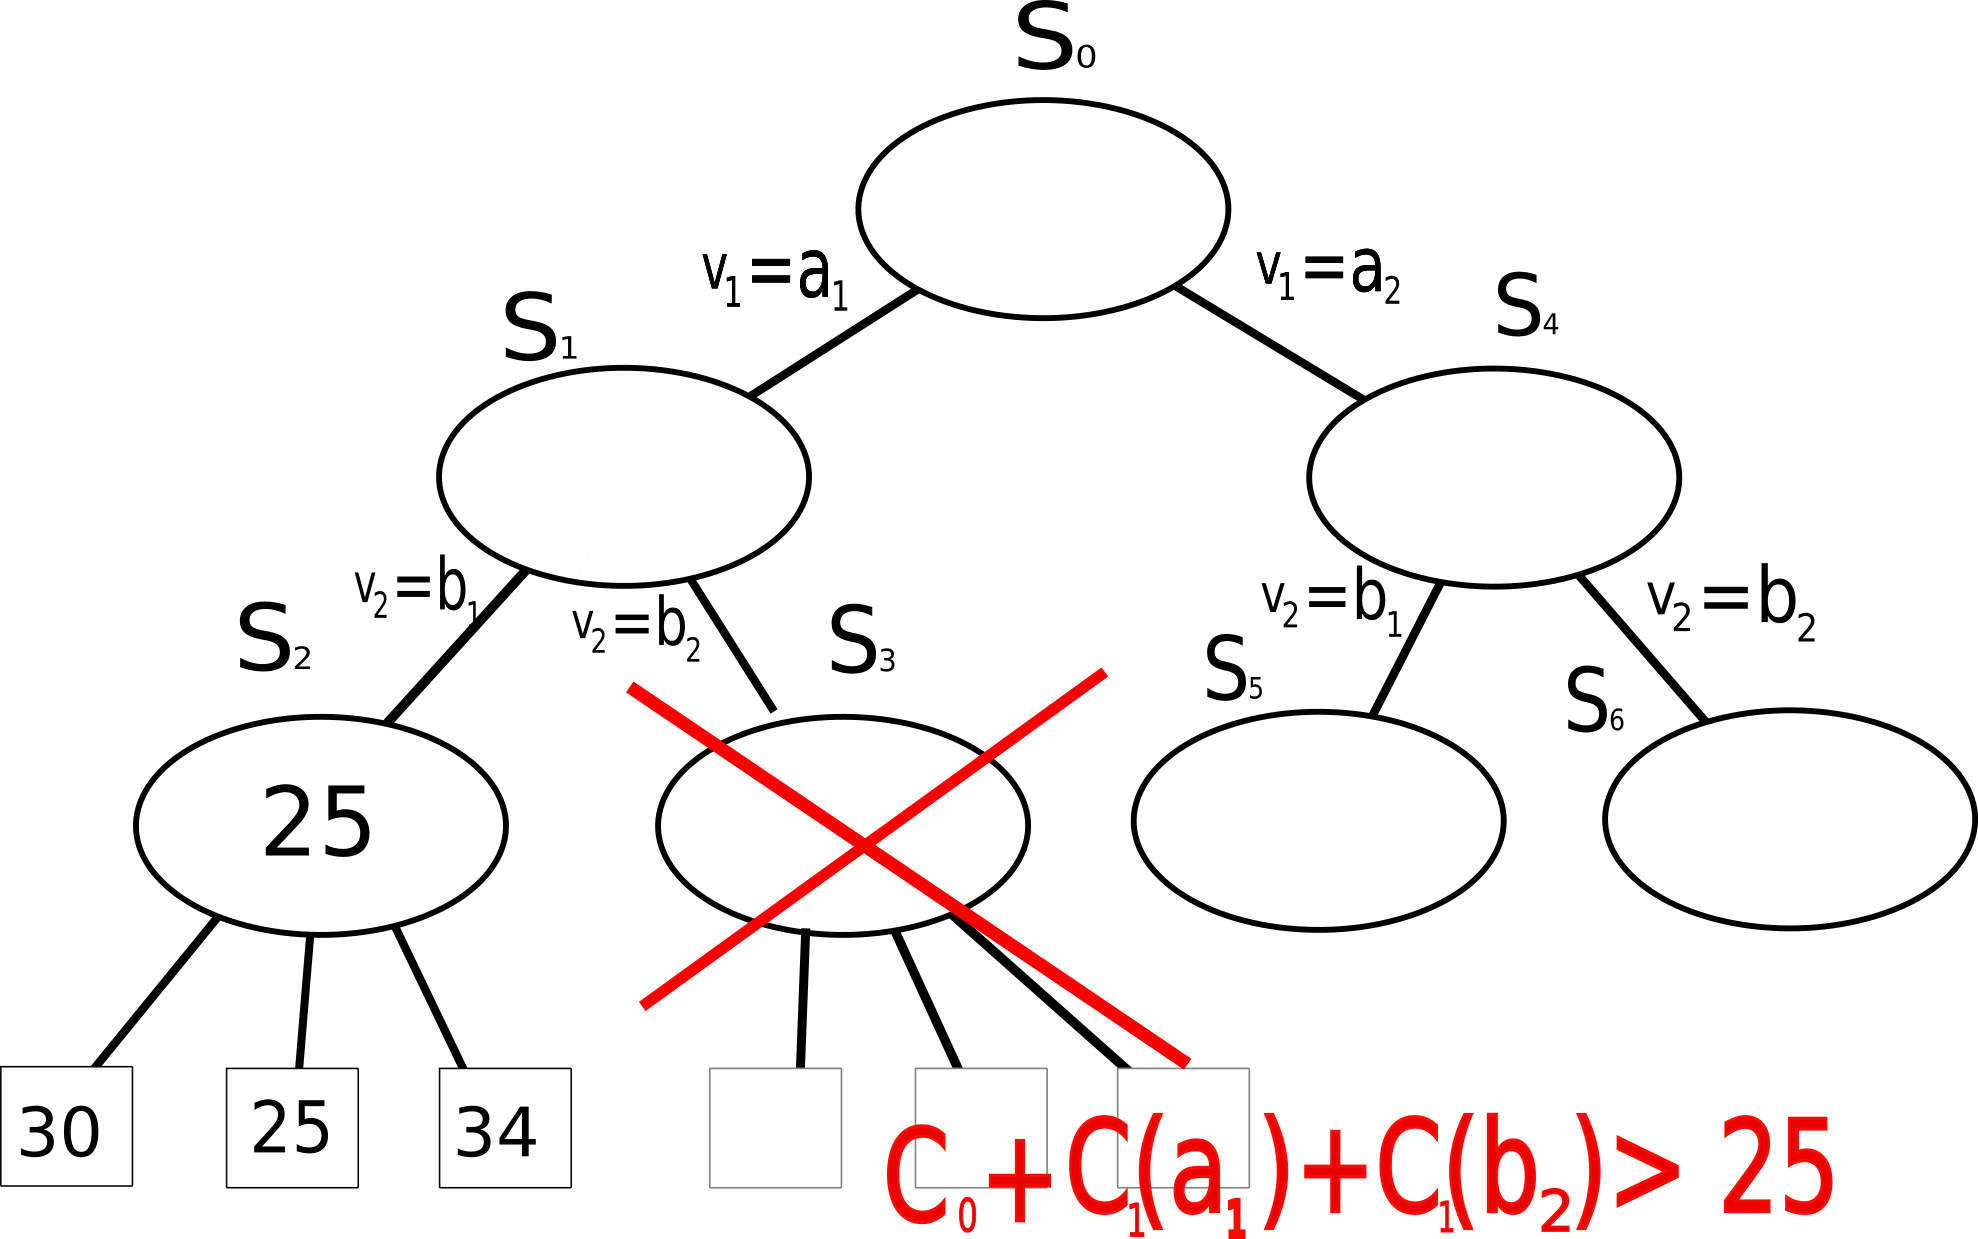
\includegraphics[width=12cm]{figure/DFBB.png} \\
  \end{tabular}
  \caption{\textbf{Principe de l'algorithme du Depth-First Branch and Bound} Les solutions d'un CFN sont représentées sous forme d'un arbre dans lequel le sommet $S_0$ représente l'ensemble des solutions et les fils $S_1$ et $S_4$ une partition de $S_0$, avec pour chacun une première variable $v_1$ fixée. Le DFBB, descend jusqu'au sommet $S_2$ qu'il peut évaluer: un minorant de $S_2$ est 25. 25 devient le nouveau majorant du GMEC. L'algorithme remonte et redescend vers $S_3$. Ici le coût constant plus le coût des affectations de $v_1$ et $v_2$ est supérieur au majorant: On peut élaguer l'arbre au sommet $S_3$.}
  \label{fig:DFBB}  
\end{figure}

\subsubsection{Equivalence Preserving Transformation}
Une EPT, ou \og Equivalence Preserving Transformation\fg, transforme un CFN $A$ en un CFN $B$ tel que pour chaque solution (chaque affectation des variables), le total des coûts  est identique. $A$ et $B$ sont dits \og en cohérence locale \fg. Le principe est de déplacer les coûts entre fonctions pour les attribuer aux fonctions les plus simples, qui portent sur une seule variable au plus (les coûts unitaires et constants). L'objectif est de faire apparaître de bons minorants pour le DFBB \cite{schiex00}. L'avantage ici, est de pouvoir conserver les transformations dans un chemin de l'arbre de recherche tout au long de l'optimisation. Il existe deux types de transformations:
\begin{itemize}
\item la première appelée projection consiste à transférer un coût de l'ensemble des coûts unaires vers le coût constant, des coûts binaires vers le coût constant ou encore des coûts binaires vers les coûts unaires.
\item le second type de transformation fait l'inverse, c'est à dire transfère un coût d'une fonction unaire vers les fonctions binaires impliquant la même valeur de variable. Une telle transformation permet une augmentation du transfert total vers le coût constant.
\end{itemize}
Un exemple inspiré de la thèse de Seydou Traoré est présenté à  la figure \ref{fig:EPT}.

\begin{figure}[!htbp]
  \centering
  \begin{tabular}{c}
    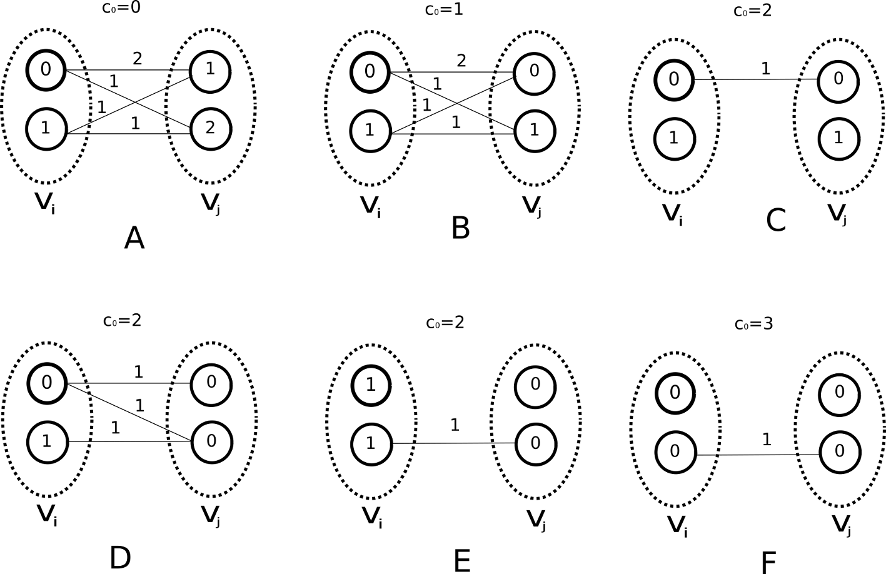
\includegraphics[width=14cm]{figure/coherence_local.png} \\
  \end{tabular}
  \caption{\textbf{Exemple de transformations EPT sur un CFN composé de 2 variables $v_i$ et $v_j$ ayant deux valeurs possibles.} La transformation de $A$ vers $B$ est une projection de $v_j$ vers le coût constant $C_0$. Puis une projection des fonctions binaires mène en $C$. La seconde valeur de $v_j$ est distribuée sur les arcs en $D$. Cela permet deux nouvelles projections qui mènent à $E$ puis à $F$. $A$ et $F$ sont en cohérence locale.}
  \label{fig:EPT}
\end{figure}

Cette approche a montré sa supériorité, avec l'outil toulbar2 \cite{Allouche14,Traore13}, par rapport à un ensemble de résolveurs de CFN parmi les plus réputés actuellement qui exploitent notamment l'approche DEE/A* ou le backtracking. Toulbar2 en combinant FFBB, EPT et DEE a été capable de trouver le GMEC dans le plus grand nombre de problèmes issu du CPD proposés aux différents outils.
\subsection{L'heuristique Multistart Steepest Descent (MSD)}
\label{MSD}
En 2000, Wernisch, Hery et Wodak \cite{Wernisch00} partent du constat que l'espace conformationnel et les fonctions d'énergie utilisées ne capturent que partiellement la réalité. Ainsi, le GMEC ne correspondra pas forcément à la séquence la plus stable. D'autre part, des protéines avec des taux d'identité de moins de $50\%$ peuvent conserver quasiment la même structure 3D. Cela révèle l'immensité du nombre de séquences-conformations propre à un pli. Ainsi, leur objectif n'est pas de résoudre un problème d'optimisation, mais d'exhiber un ensemble de séquences de basse énergie. Ils proposent alors une heuristique conçue pour le CPD. Il s'agit d'une procédure simple qui produit une grande quantité de séquences-conformations de basse énergie, sans se focaliser sur le GMEC.

Un cycle heuristique se déroule de la façon suivante. Au départ, une séquence-conformation est construite en attribuant de façon aléatoire un type d'acide aminé et un rotamère à chaque position de la chaîne. Ensuite, en parcourant la séquence du début jusqu'à la fin, l'algorithme procède par des ajustements successifs à chaque position. Pour chaque position $i$ de la séquence, tous les états possibles sont évalués, le reste de la séquence et des rotamères étant fixés. Le meilleur rotamère est alors attribué en $i$, puis on passe à la position suivante. La séquence est ainsi ajustée par plusieurs passages successifs, jusqu'à convergence de l'énergie, voir l'algorithme \ref{alg:MSD}. Un cycle est très rapide, ce qui permet de produire dans les cas usuels, plusieurs milliers de séquences par heure. L'utilisation mémoire hormis le stockage des énergies est quasi nulle. Il n'impose pas que la fonction d'énergie soit décomposable par paires, mais il s'en accommode très bien, en rendant possible l'utilisation de la mémoire par bloc pour l'ensemble des énergies impliquant une position $i$ donnée.

\begin{algorithm}
  \For{chaque cycle heuristique}{ 
    choisir une séquence-conformation $C$ aléatoirement \;
    \While{  l'énergie de $C$ est améliorée }{
      \For{  $i$ allant de la première position de $C$ jusqu'à la dernière}{
        fixer $C$ sauf à la position i \;
        déterminer le meilleur rotamère possible en i  \;
        fixer $C$ en $i$ avec ce rotamère \;
      }
    }
    sauvegarder  C \;
  }
  \caption{L'algorithme Multistart Steepest Descent}\label{alg:MSD}
\end{algorithm}


\subsection{L'algorithme génétique}

Holland et ces collaborateurs \cite{Goldberg88} introduisent une nouvelle approche inspirée des principes biologiques de la sélection naturelle, avec des opérations comme des mutations, des croisements et la sélection. L'algorithme génétique a pour objectif d'obtenir un ensemble de solutions proches de l'optimum en un temps raisonnable.
Le schéma général est le suivant. Une population de séquences-conformations est générée de façon aléatoire. L'énergie de tous les membres de la population est évaluée. Une sélection basée sur l'énergie est appliquée, ce qui diminue la taille de la population. Des mutations aléatoires et des croisements sont appliqués à la nouvelle population, qui augmente. Enfin, une condition d'arrêt est évaluée. Si elle n'est pas réalisée, l'algorithme retourne à l'étape d'évaluation (voir la figure \ref{fig:algo_gene}). 

\begin{figure}[!h]
  \centering
  \begin{tabular}{c}
    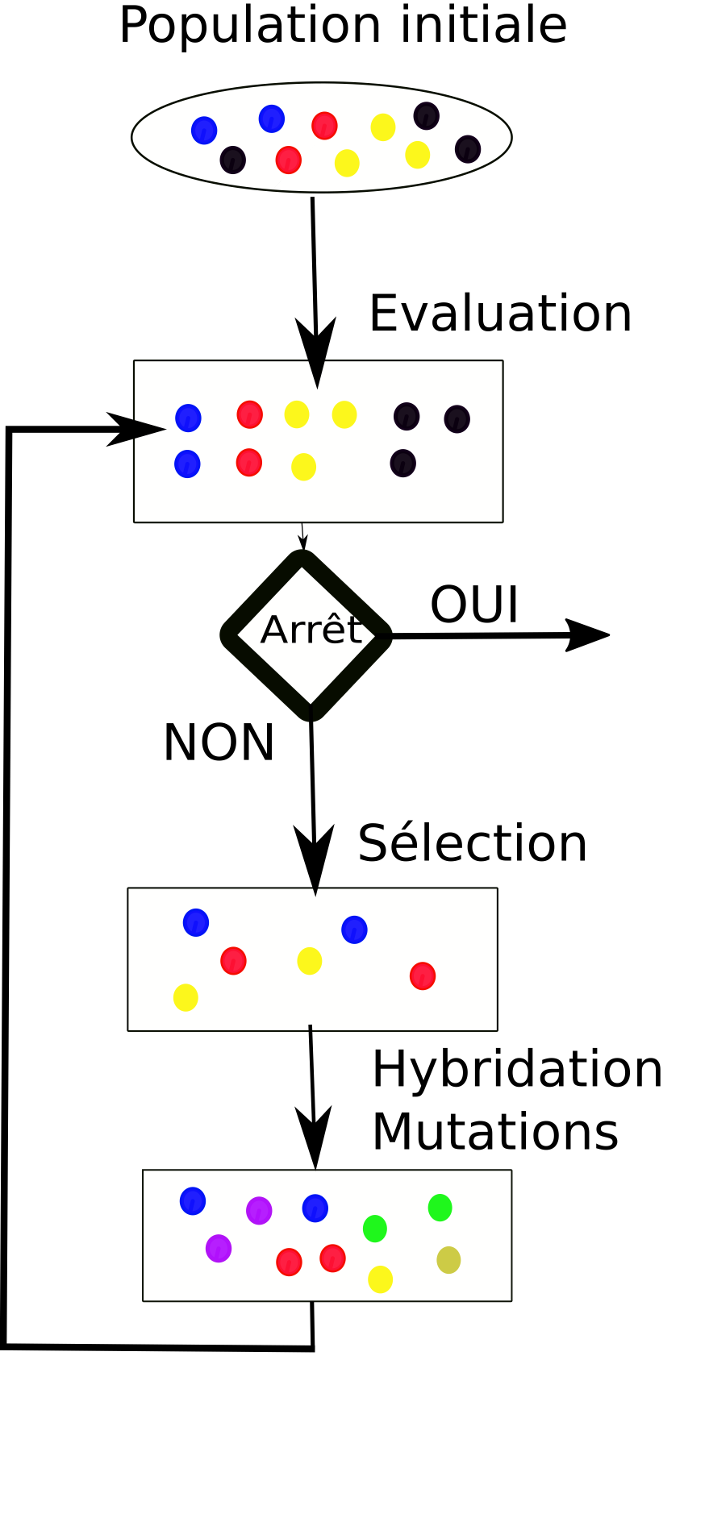
\includegraphics[width=5cm]{figure/algo_genetique.png} \\
  \end{tabular}
  \caption{\textbf{L'algorithme génétique}}
  \label{fig:algo_gene}
\end{figure}


L'individu de meilleure énergie au sein de la population tend à se reproduire le plus vite. Donc la valeur moyenne de l'énergie de l'ensemble des séquences-conformations converge. On peut voir ici que le nombre de membres de la population est un paramètre de l'algorithme. Plus ce nombre est faible plus la convergence va être rapide. A contrario, plus ce nombre est grand, meilleure est l'exploration de l'espace d'états. Les atouts de l'algorithme génétique sont sa capacité à franchir des barrières énergétiques par des changements de séquences rapides via des croisements et sa capacité à optimiser en parallèle différents secteurs de la structure.

\subsection{Le Monte Carlo}
\label{sub:MC}
Dans son acceptation la plus générale, un algorithme Monte Carlo est un algorithme stochastique (il utilise une source de hasard) qui approche probablement la solution exacte en un temps d'exécution déterminable a priori. Cela le distingue, parmi les algorithmes stochastiques, d'un algorithme de Las Vegas qui donne un résultat exact dans un temps d'exécution non déterministe, et d'un algorithme d'Atlantic City qui donne des résultats probablement corrects dans un temps probablement rapide. Parmi les algorithmes Monte Carlo, les algorithmes Monte Carlo par Chaînes de Markov (MCMC) ont été particulièrement étudiés. Ce ne sont pas des algorithmes d'optimisation, mais des algorithmes d'échantillonnage d'une distribution de probabilité $\pi$. On veut générer des éléments $x_i$ de l'espace des phases tels que la distribution $D=\{x_i,\ i \in \mathbb{N} \}$ converge vers $\pi$ (dans un sens mathématique à préciser).

Il existe plusieurs méthodes pour répondre à cette question, mais les MCMC sont bien adaptés aux situations où l'espace des états est de grande dimension. Un autre avantage des algorithmes MCMC est qu'elles ne nécessitent pas la connaissance de la constante de normalisation de $\pi$. Cela constitue un attrait important parce que dans beaucoup de situations cette constante de normalisation est particulièrement difficile à calculer. Pour ces raisons, l'échantillonnage par MCMC est très populaire depuis plus de cinquante ans. Dans la suite, nous donnons des conditions suffisantes pour que ce type l'algorithme converge dans le cadre d'un espace d'états $E$ fini, puis nous détaillons le plus célèbre d'entre eux, l'algorithme de Metropolis-Hasting. L'idée est de générer un élément $x_i$ en utilisant dans les états déjà visités uniquement $x_{i-1}$. Ce type de processus, où la mémoire utilisée est réduite à l'état précédent caractérise les processus de Markov.


On appelle processus stochastique, une suite de variables aléatoires $\{X_n\}$ à valeurs dans $E$.
Une chaîne de Markov est un processus stochastique tel que:\\
\[ \forall n \geqslant 0 ,\ \forall (x_0,,..,x_{n-1},x) \in E^{n+1},\  P(X_n=x|X_{n-1}=x_0,..,X_{0}=x_{n-1}) = P(X_n=x|X_{n-1}=x_0) \]
Une chaîne de Markov est homogène si:
\begin{equation}
  \label{eq_homog}
\forall n \geqslant 0 ,\ \forall x_i,x_j \in E,\ P(X_n=x_i|X_{n-1}=x_j)= P(X_{n+1}=x_i|X_n=x_j) 
\end{equation}
C'est-à-dire que la probabilité de transition $P$ est indépendante de $n$. Dans la suite, on ne considère que des chaînes de Markov homogènes et on note:
\[P(X_n=a | X_{n-1}=b) = P(a|b)\]
Pour simplifier les notations, on introduit une matrice de transition $P$ avec $P_{ab}=P(X_1=b|X_0=a)$ et on écrit
$\mu_0 =(P(X_0=a))_{a \in E}$ et $\mu_1 =(P(X_1=a))_{a \in E}$. On a alors:
\[\mu_1 =P \mu_0\] 

\subsubsection{Le principe de la balance détaillée}

Le principe de la balance détaillée est un principe général de comportement des systèmes dynamiques. Il a été utilisé par Boltzmann pour la construction de la physique statistique et Cercignani et Lampis ont montré qu'il était vrai pour les gaz polyatomiques \cite{Cercignani81}. Il peut s'exprimer de la façon suivante. Pour un système dynamique $\mathcal{S}$ à l'équilibre, $a$ et $b$ deux éléments de l'espace des phases associé à $\mathcal{S}$, la probabilité de transition de $a$ vers $b$ est égale à la probabilité de transition de $b$ vers $a$, ou encore: 
\begin{equation}
\forall a,b \in \mathcal{S},\ \mathcal{P}(a \rightarrow b) = \mathcal{P}(b \rightarrow a) 
\end{equation}
Pour pouvoir appliquer ce principe aux chaînes de Markov, introduisons une définition proche. Soit $q$ une probabilité sur $E$. Une chaîne de Markov est dite réversible par rapport à $q$ si
\begin{equation}
\forall a,b \in E,\ q(b)P(a|b)=q(a)P(b|a)
\end{equation}
On a alors:
\begin{equation}
\forall a \in E,\ P q(a) = \sum_{b \in E} q(b)P(a|b) = \sum_{b \in E} q(a)P(b|a) = q(a) \sum_{b \in E}P(b|a) = q(a)
\end{equation}
Ainsi, la probabilité $q$ est inchangée après la transition $P$, la chaîne est dite stationnaire pour $q$.

Il nous faut alors construire une chaîne de Markov réversible pour la distribution cible $\pi$. Mais cela ne suffit pas. En effet, même si $\{X_n\}$ est stationnaire pour $\pi$, rien ne dit que la chaîne va, à un moment, distribuer les états comme $\pi$. Se pose la question de la convergence vers $\pi$. Or, si $E$ est discret, une chaîne de Markov réversible est dîte ergodique si et seulement si:
\begin{itemize}
\item Pour tous $a$ et $b$ de l'espace d'états il existe un chemin de $a$  vers $b$  de probabilité non nulle. 
\item Il n'existe pas de $a$ de $E$ tel que la chaîne revienne en $x$ périodiquement.
\item  Au cours du temps, tous les états sont visités par la chaîne avec une probabilité non nulle. 
\end{itemize}
On a alors, le résultat suivant: une chaîne ergodique converge vers son unique distribution stationnaire.

\subsubsection{L'algorithme de Metropolis}

Nous pouvons maintenant décrire l'algorithme de Metropolis-Hastings. L'idée initiale de Metropolis est de construire un l'algorithme qui échantillonne la distribution de Boltzmann. Elle donne la probabilité d'un état $x_i$ du système en fonction de son énergie et de la température:

\begin{equation}
  \label{eq:Boltzmann}
\pi(x_i) = \frac{\exp(-\beta E_{x_i})}{\sum_{x_j \in E}\exp(-\beta E_{x_j})} 
\end{equation}
avec $\beta = \frac{1}{kT}$, $E_{x_i}$  l'énergie de $x_i$, $T$ la température et $k$ la constante de Boltzmann. La constante de normalisation de la probabilité s'appelle la fonction de partition du système. Elle est particulièrement difficile à calculer.

On définit alors la probabilité de transition $P$ comme le produit de deux probabilités:
\begin{equation}
  \label{decomp_Metro}
P (x_j|x_i) = sel(x_j|x_i)acc(x_j|x_i)
\end{equation}
avec $sel$ une probabilité de sélectionner l'état $x_j$ de $E$ lorsque le système est dans l'état $x_i$ et $acc$ la probabilité d'accepter l'état $x_j$ étant en $x_i$. Si la chaîne respecte le principe de la balance détaillée par rapport à $\pi$, on a:
\begin{equation}
  \label{balance}
\pi(x_i)sel(x_j|x_i)acc(x_j|x_i) = \pi(x_j)sel(x_i|x_j)acc(x_i|x_j) 
\end{equation}
Si on se limite à une probabilité de sélection symétrique:
\begin{equation}
    \label{bd_Metropolis}
\pi(x_i)acc(x_j|x_i) = \pi(x_j)acc(x_i|x_j) 
\end{equation}
ce qui équivaut à
\begin{equation}
\frac{acc(j|i)}{acc(i|j)} =\frac{\pi(j)}{\pi(i)} = \frac{\exp(-\beta E_{x_j})}{\exp(-\beta E_{x_i})} = \exp(-\beta \Delta E) 
\end{equation}\\
avec $\Delta E =  E_{x_j} - E_{x_i}$. Ainsi, le calcul de la fonction de partition est évité! Métropolis propose alors la probabilité d'acceptation suivante: 
\begin{equation}
acc(x_i|x_j) = \exp(- \beta \Delta E)\ \text{si}\ \Delta E >0;\ acc(x_i|x_j)=1\ \text{sinon}
\end{equation}
On a bien: 
\begin{equation}
\forall\ x_i, x_j \in E,\ \frac{acc(x_j|x_i)}{acc(x_i|x_j)} = \exp(\beta \Delta E)
\end{equation}\\
Il suffit alors de choisir une probabilité de sélection symétrique ne violant pas les conditions ergodiques pour obtenir notre convergence. Par la suite, Hastings généralise l'algorithme à une probabilité $sel()$ non symétrique en choisissant acc() telle que:
\begin{equation}\label{eq:Hasting}
acc(x_i|x_j) = \exp(-\beta \Delta E) \frac{sel(x_j|x_i)}{sel(x_i|x_j)}\ \text{si}\ \Delta E >0;\ acc(x_i|x_j)=1\ \text{sinon}
\end{equation}
Si l'on injecte cette nouvelle probabilité dans l'équation \ref{balance}, on a encore le respect de la balance détaillée et la convergence. La séquence d'instructions est résumée par l'algorithme \ref{alg:Metro}. Dans toute la suite, l'algorithme Monte Carlo (MC) désigne l'algorithme de Metropolis-Hastings, ce qui est un usage courant.

\begin{algorithm}
  Une séquence-conformation $S_0$ est choisie aléatoirement\;
  \For{ chacun des  pas $i$ de la trajectoire}{
    choisir une proposition  $S'_i$ à partir d'une probabilité conditionnelle sel(.,S)\;
    calculer une probabilité d'acceptation acc;
    \If{$acc \geq 1$}{
      $S_{i +1} = S_i'$ \;
      sauvegarder  $S_{i+1}$ \;
      }
    \Else{
      alors       $S_{i +1} = S_i'$ avec une probabilité acc\;
      sauvegarder  $S_{i+1}$ \;
      \Else {
        $S_{i+1} = S_i$
      }
     }
    }
\caption{L'algorithme de Metropolis} \label{alg:Metro}
\end{algorithm}


\subsection{Le Monte Carlo avec échanges de répliques (REMC)}
\label{REMC}

Une amélioration de l'algorithme de Métropolis-Hastings, connu sous le nom de \og Replica Exchange Monte Carlo\fg a été introduite par Swendsen and Wang \cite{Swendsen86}. La méthode est également connue sont le nom \og parallel tempering\fg. L'objectif est d'accélérer la convergence en permettant au processus stochastique de visiter plusieurs zones énergétiques simultanément. Ainsi, l'algorithme couple l'exploration des bassins de basses énergies proches de l'optimum, avec l'exploration des zones de plus hautes énergies, ce qui facilite la sortie des minimums locaux.

On considère $N$ simulations MC du système à $N$ températures. Ces répliques du système sont indépendantes les unes par rapport aux autres. On note $T_m$ avec $m=1,..,N$ les températures. Toutes ces températures sont différentes et il y a toujours une réplique à chaque température. Ainsi, nous nous plaçons dans un ensemble généralisé noté $E^N$, constitué des $N$-uplets $(x_1,...,x_n)$ avec les $x_i$ éléments de $E$, et $1 \leqslant i \leqslant N$  indexant les répliques. On travaille avec une chaîne de Markov $\{X(t),\ t \in \mathbb{N}\}$ , avec $X(t)=(x_1(t),...,x_n(t))$ une variable aléatoire à valeur dans $E^N$ au temps $t$. On ajoute maintenant un nouveau type de déplacement, qui consiste à intervertir au temps $t$ l'état $x_i$ de la simulation à la température $T_i$ avec l'état $x_{i+1}$ à la température $T_{i+1}$. On a alors:
\begin{equation}
  \label{REMC_move}
\begin{cases}
& x_{i+1}(t+1)=x_i(t)\\
& \ \ \ x_{i}(t+1)=x_{i+1}(t)
\end{cases}
\end{equation}
L'algorithme consiste alors à effectuer de façon itérative:
\begin{itemize}
\item un ensemble de $k$ déplacements de type MC, avec $k$ une constante  
\item une tentative de déplacement de type \ref{REMC_move} 
\end{itemize}
Pour que le processus respecte la balance détaillée, le nouveau déplacement doit respecter certaines conditions. Nous introduisons une probabilité d'acceptation $acc_{swap}$ spécifique. Pour la déterminer, nous reprenons la même démarche que pour le Monte Carlo simple. Comme les répliques sont sans interactions, la distribution cible de la chaîne de Markov est égale aux produits des distributions cibles aux différentes températures:
\begin{equation}
\pi(X)=\frac{1}{Z} \exp(-\sum_{i=1}^N \frac{E_{x_i}}{kT_i})
\end{equation}
En injectant cette expression de $\pi^$ et les équations \ref{REMC_move} dans \ref{bd_Metropolis}, on obtient:
\begin{displaymath}
\frac{acc_{swap}(X(t+1)|X(t))}{acc_{swap}(X(t)|X(t+1))} =\frac{\pi(X(t))}{\pi(X(t+1))}
                                                     = \frac{ \exp(-E_{x_i}/kT_i) \exp(-E_{x_{i+1}}/kT_{i+1})}{\exp(-E_{x_{i+1}}/kT_i) \exp(-E_{x_i}/kT_{i+1})} 
                                                       = \exp(-\Delta) 
\end{displaymath}
avec $\Delta = (\frac{1}{kT_i} -\frac{1}{kT_{i+1}})(E_{x_i} - E_{x_{i+1}})$. \\
Ceci peut être satisfait par le critère de Metropolis:
\begin{displaymath}
acc_{swap}(X(t+1)|X(t)) = \exp(- \Delta)\ \text{si}\ \Delta >0;\ acc_{swap}(X(t+1)|X(t)) = 1\ \text{sinon}\ 
\end{displaymath}
Le REMC peut alors se décrire comme l'algorithme \ref{algoREMC}.

\begin{algorithm}

  Lancement en parallèle de $N$ marcheurs Monte Carlo aux températures ordonnées $(t_1,...,t_n)$ \;
\For{ les pas $p$ multiples d'une constante $P$}{
choisir aléatoirement $i$ compris entre $1$ et $N-1$, ce qui sélectionne les marcheurs aux températures $t_i$ et $t_{i+1}$ \;
la probabilité d'acceptation acc_{swap} est calculée \;
\If{$acc_{swap} \geq 1$}{
  Les marcheurs échangent leur température \;
  \Else
      {
        Les marcheurs échangent leur température , avec la probabilité acc_{swap} \;
      }
  }
}
\caption{L'algorithme REMC}\label{algoREMC}
\end{algorithm}


Il reste au simulateur à adapter le nombre de répliques, les températures utilisées et la fréquence des tentatives d'échange à sa problématique. La capacité de REMC à être exécuté sur des machines parallèles à entrainé sa grande popularité, en particulier dans le domaine de la modélisation moléculaire, mais aussi en physique, chimie, intelligence artificielle.

%%% Local Variables:
%%% mode: latex
%%% TeX-master: "../these"
%%% End:
